\chapter{Gamma detection testing}
The purpose of this experiment is to determine the conditions necessary for selected photodiodes to be used as detectors for gamma spectroscopy. Note that some of the selected photodiodes are not intended to be used as gamma-ray detectors. The determination of the detection efficiency will be precisely done in the following chapters. 
\par
For the very first test of the photodiodes, we assembled a spectrometric setup consisting of ORTEC modules including a preamplifier ORTEC142A, a shaping amplifier 575A and a high voltage power supply 556 inside the ORTEC minibin (figure \ref{minibin}). The pulses were captured by ORTEC's EASY-MCA-2K connected to a PC running the MAESTRO Multichannel Analyzer Emulation Software \cite{maestro}. As radioactive source we used $^{57}$Co 50 mCi Mössbauer source (date of production: 3.11. 2016) and therefore it was also necessary to cover the part with radiation source with lead shielding blocks.
%The purpose of this experiment is to determine the conditions necessary for selected photodiodes to be used as detectors for gamma spectroscopy. Note that some of the selected photodiodes are not determined to be used as gamma ray detectors. The determination of the detection efficiency is precisely done in the following chapters. 
%\par
%For the very first test of photodiodes we assembled a spectrometric setup from ORTEC modules including preamplifier ORTEC142A, shaping amplifier 575A and high voltage power supply 556 inside the ORTEC minibin (figure \ref{minibin}). The pulses were captured by EASY-MCA-2K from ORTEC connected to PC running the MAESTRO Multichannel Analyzer Emulation Software \cite{maestro}. As a radioactive source we used $^{57}$Co 50 mCi Mössbauer source (date of production: 3.11. 2016) and thus it was also necessary to cover the part with radiation source with lead shielding blocks.


\begin{figure}[H]
 \centering
 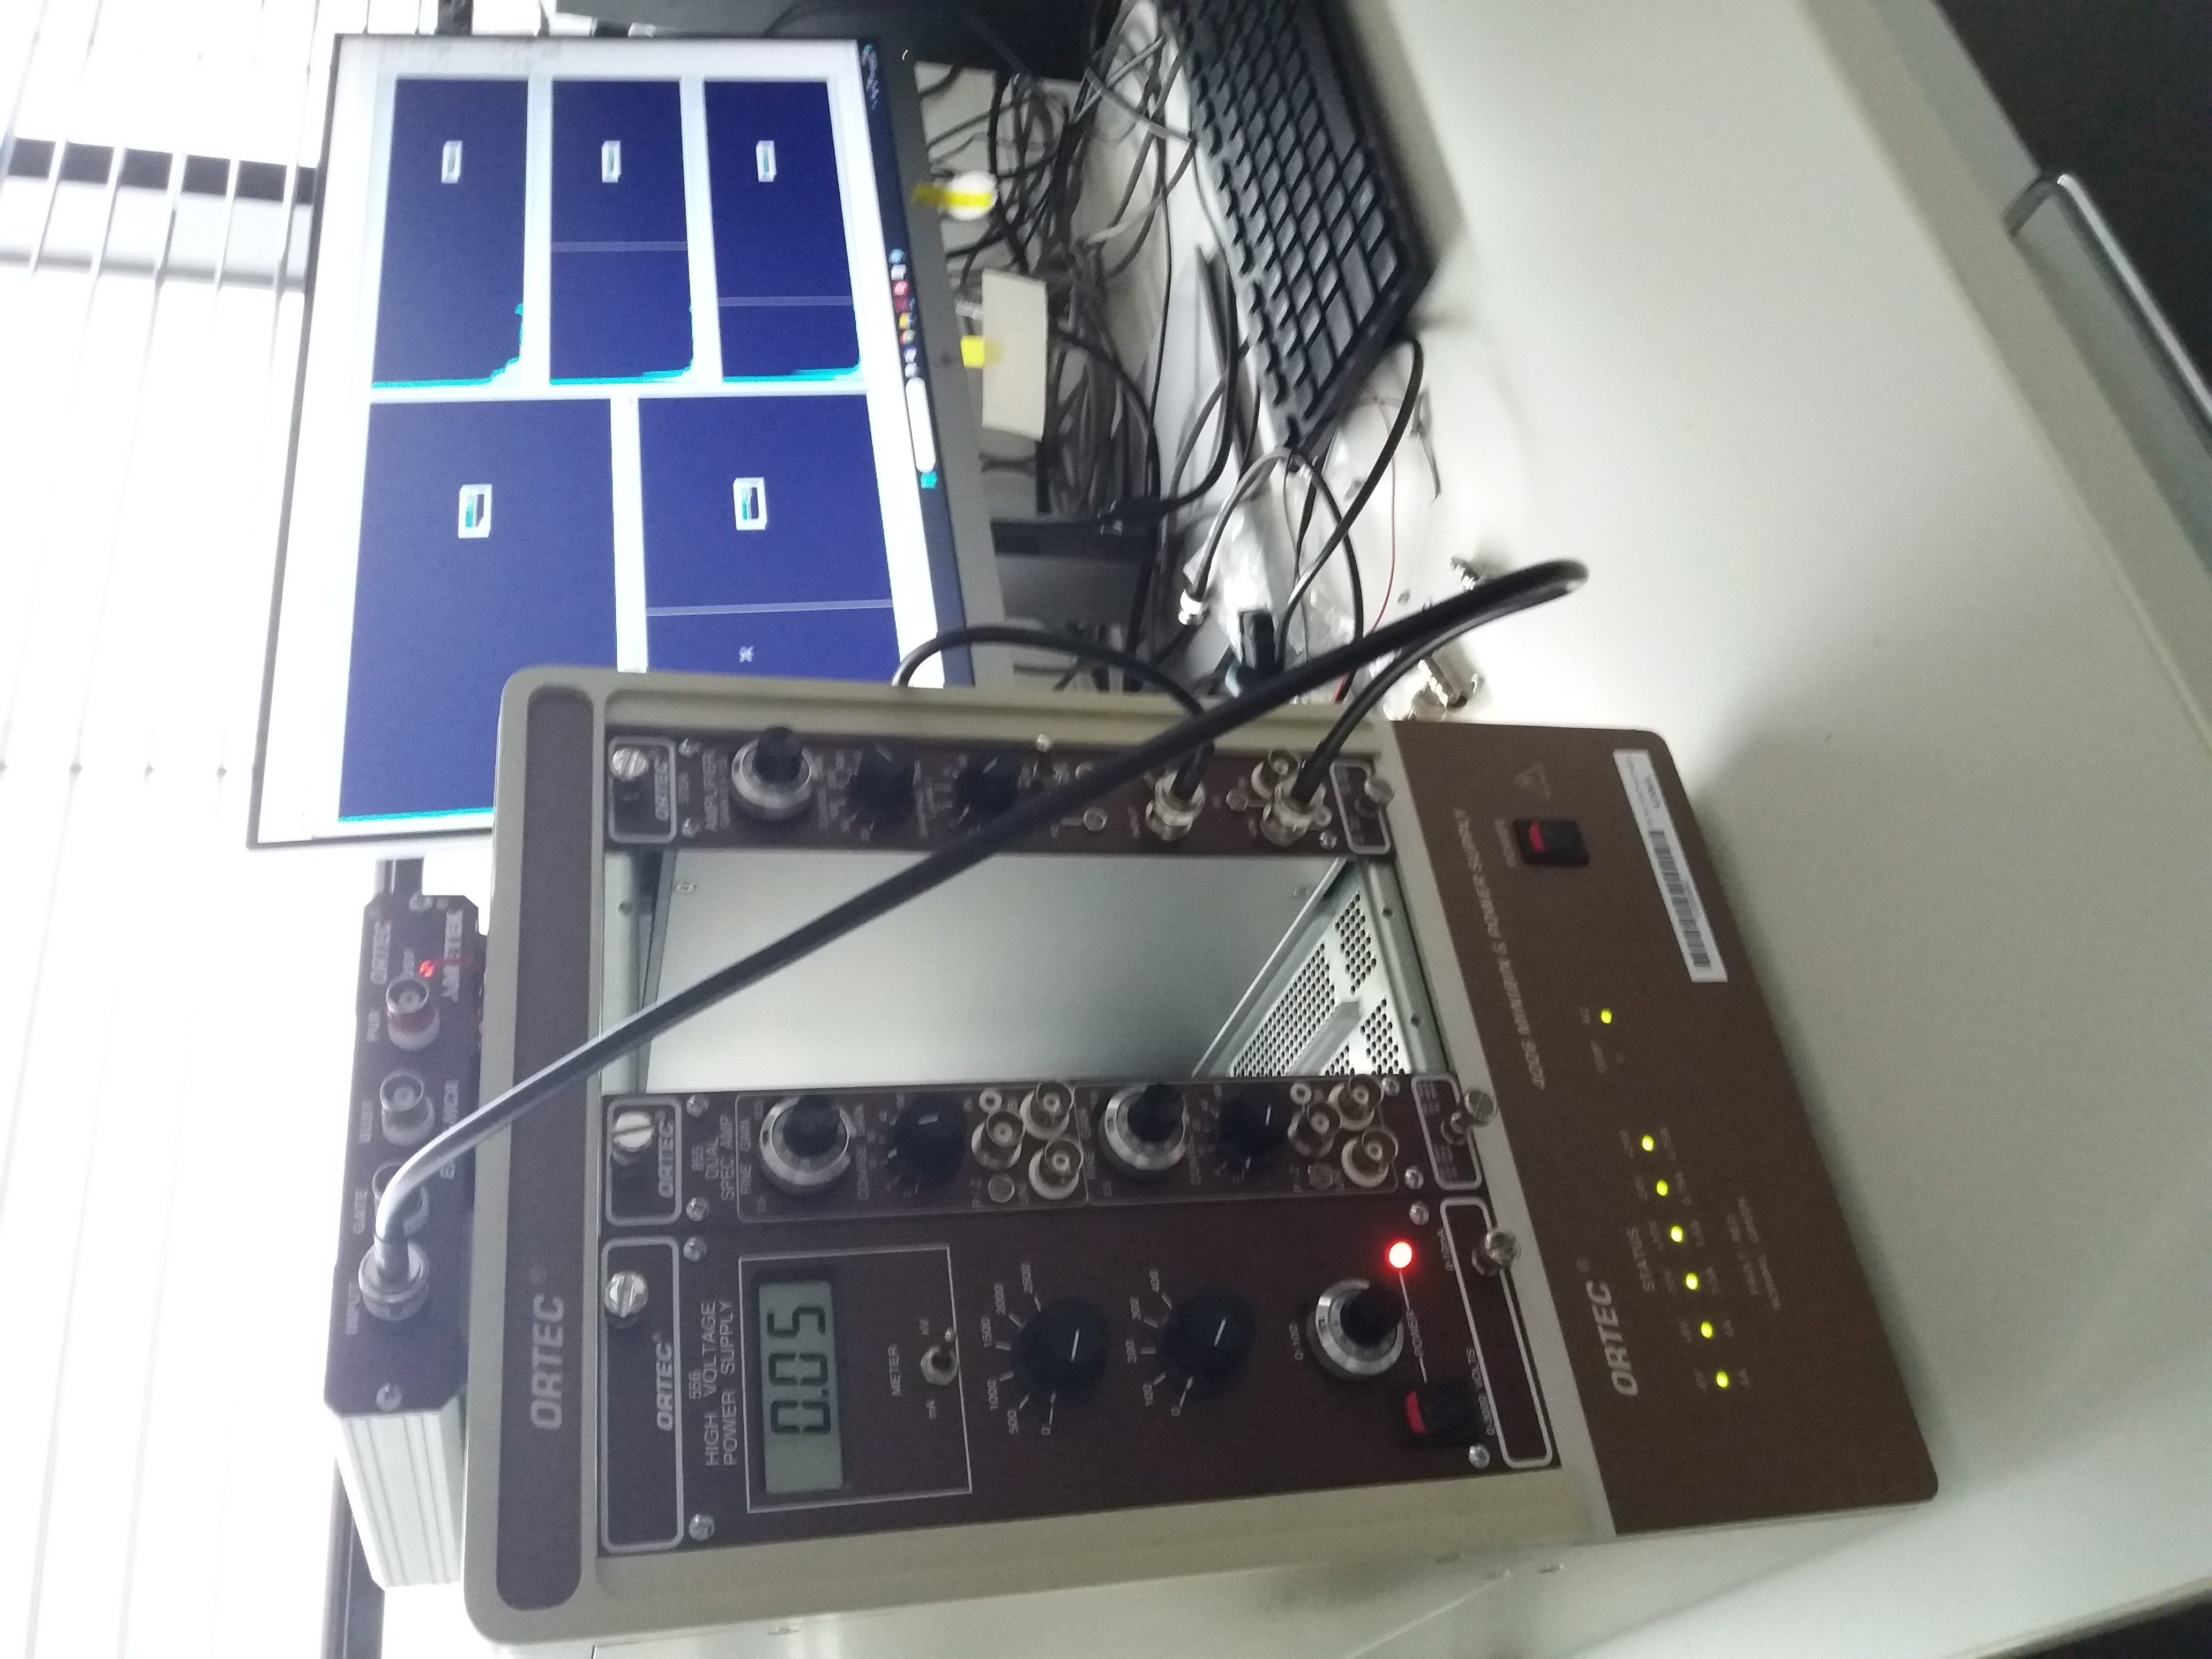
\includegraphics[scale=0.09, angle = 270]{./pictures/ORTECbin.jpg}
 \caption{ORTEC minibin with Easy MCA connected to PC.}
 \label{minibin}
 
\end{figure}


\section{Noise reduction}
When performing gamma spectroscopy measurements, the energy spectra are affected by noise. To reduce the noise as much as possible, two approaches have been tested - shielding the detector in various ways and cooling it.
%When performing gamma spectroscopy measurements, the energy spectra are affected by noise. In order to reduce noise as much as possible, two approaches were tested - shielding the detector by various ways and cooling.
\subsection{Electromagnetic noise reduction}
Photodiodes must be adequately shielded from electromagnetic interference and their distance from the preamplifier input should be as short as possible. The use of poorly shielded diodes leads to high levels of electromagnetic noise, which makes a large part of the energy spectrum unobservable.
\par
Based on many tests, it has been proven that the optimal way to shield the photodiode is to place it in an aluminium box (see figure \ref{crate}). This crate must be as small as possible and connected to the ground potential. However, the front of the crate must be open to allow sufficient transmission of gamma photons to the detector. To preserve the shielding properties, this hole has to be covered with a conductive material. We chose a thin aluminium foil, which has sufficient gamma transmission parameters as well as electromagnetic shielding parameters.
%Photodiodes have to be sufficiently electromagnetically shielded and their distance to the preamplifier input should be as short as possible. Using the diodes with poor shielding leads into high levels of electromagnetic noise, which makes major part of energetic spectra unobservable.
%\par
%Based on many test it was proven that  the optimal way to shield the photodiode is to put it into the aluminium crate (see Figure \ref{crate}). This crate has to be as small as possible and has to be connected to the grounding potential. However, the front side of the crate has to be open to allow the sufficient transmission of gamma photons to the detector. To preserve the shielding properties, this drilled hole has to be still covered by a conductive material. Our choice was a thin aluminium foil, which has sufficient gamma transmission parameters as well as electromagnetic shielding parameters.

\begin{figure}[H]
 \centering
 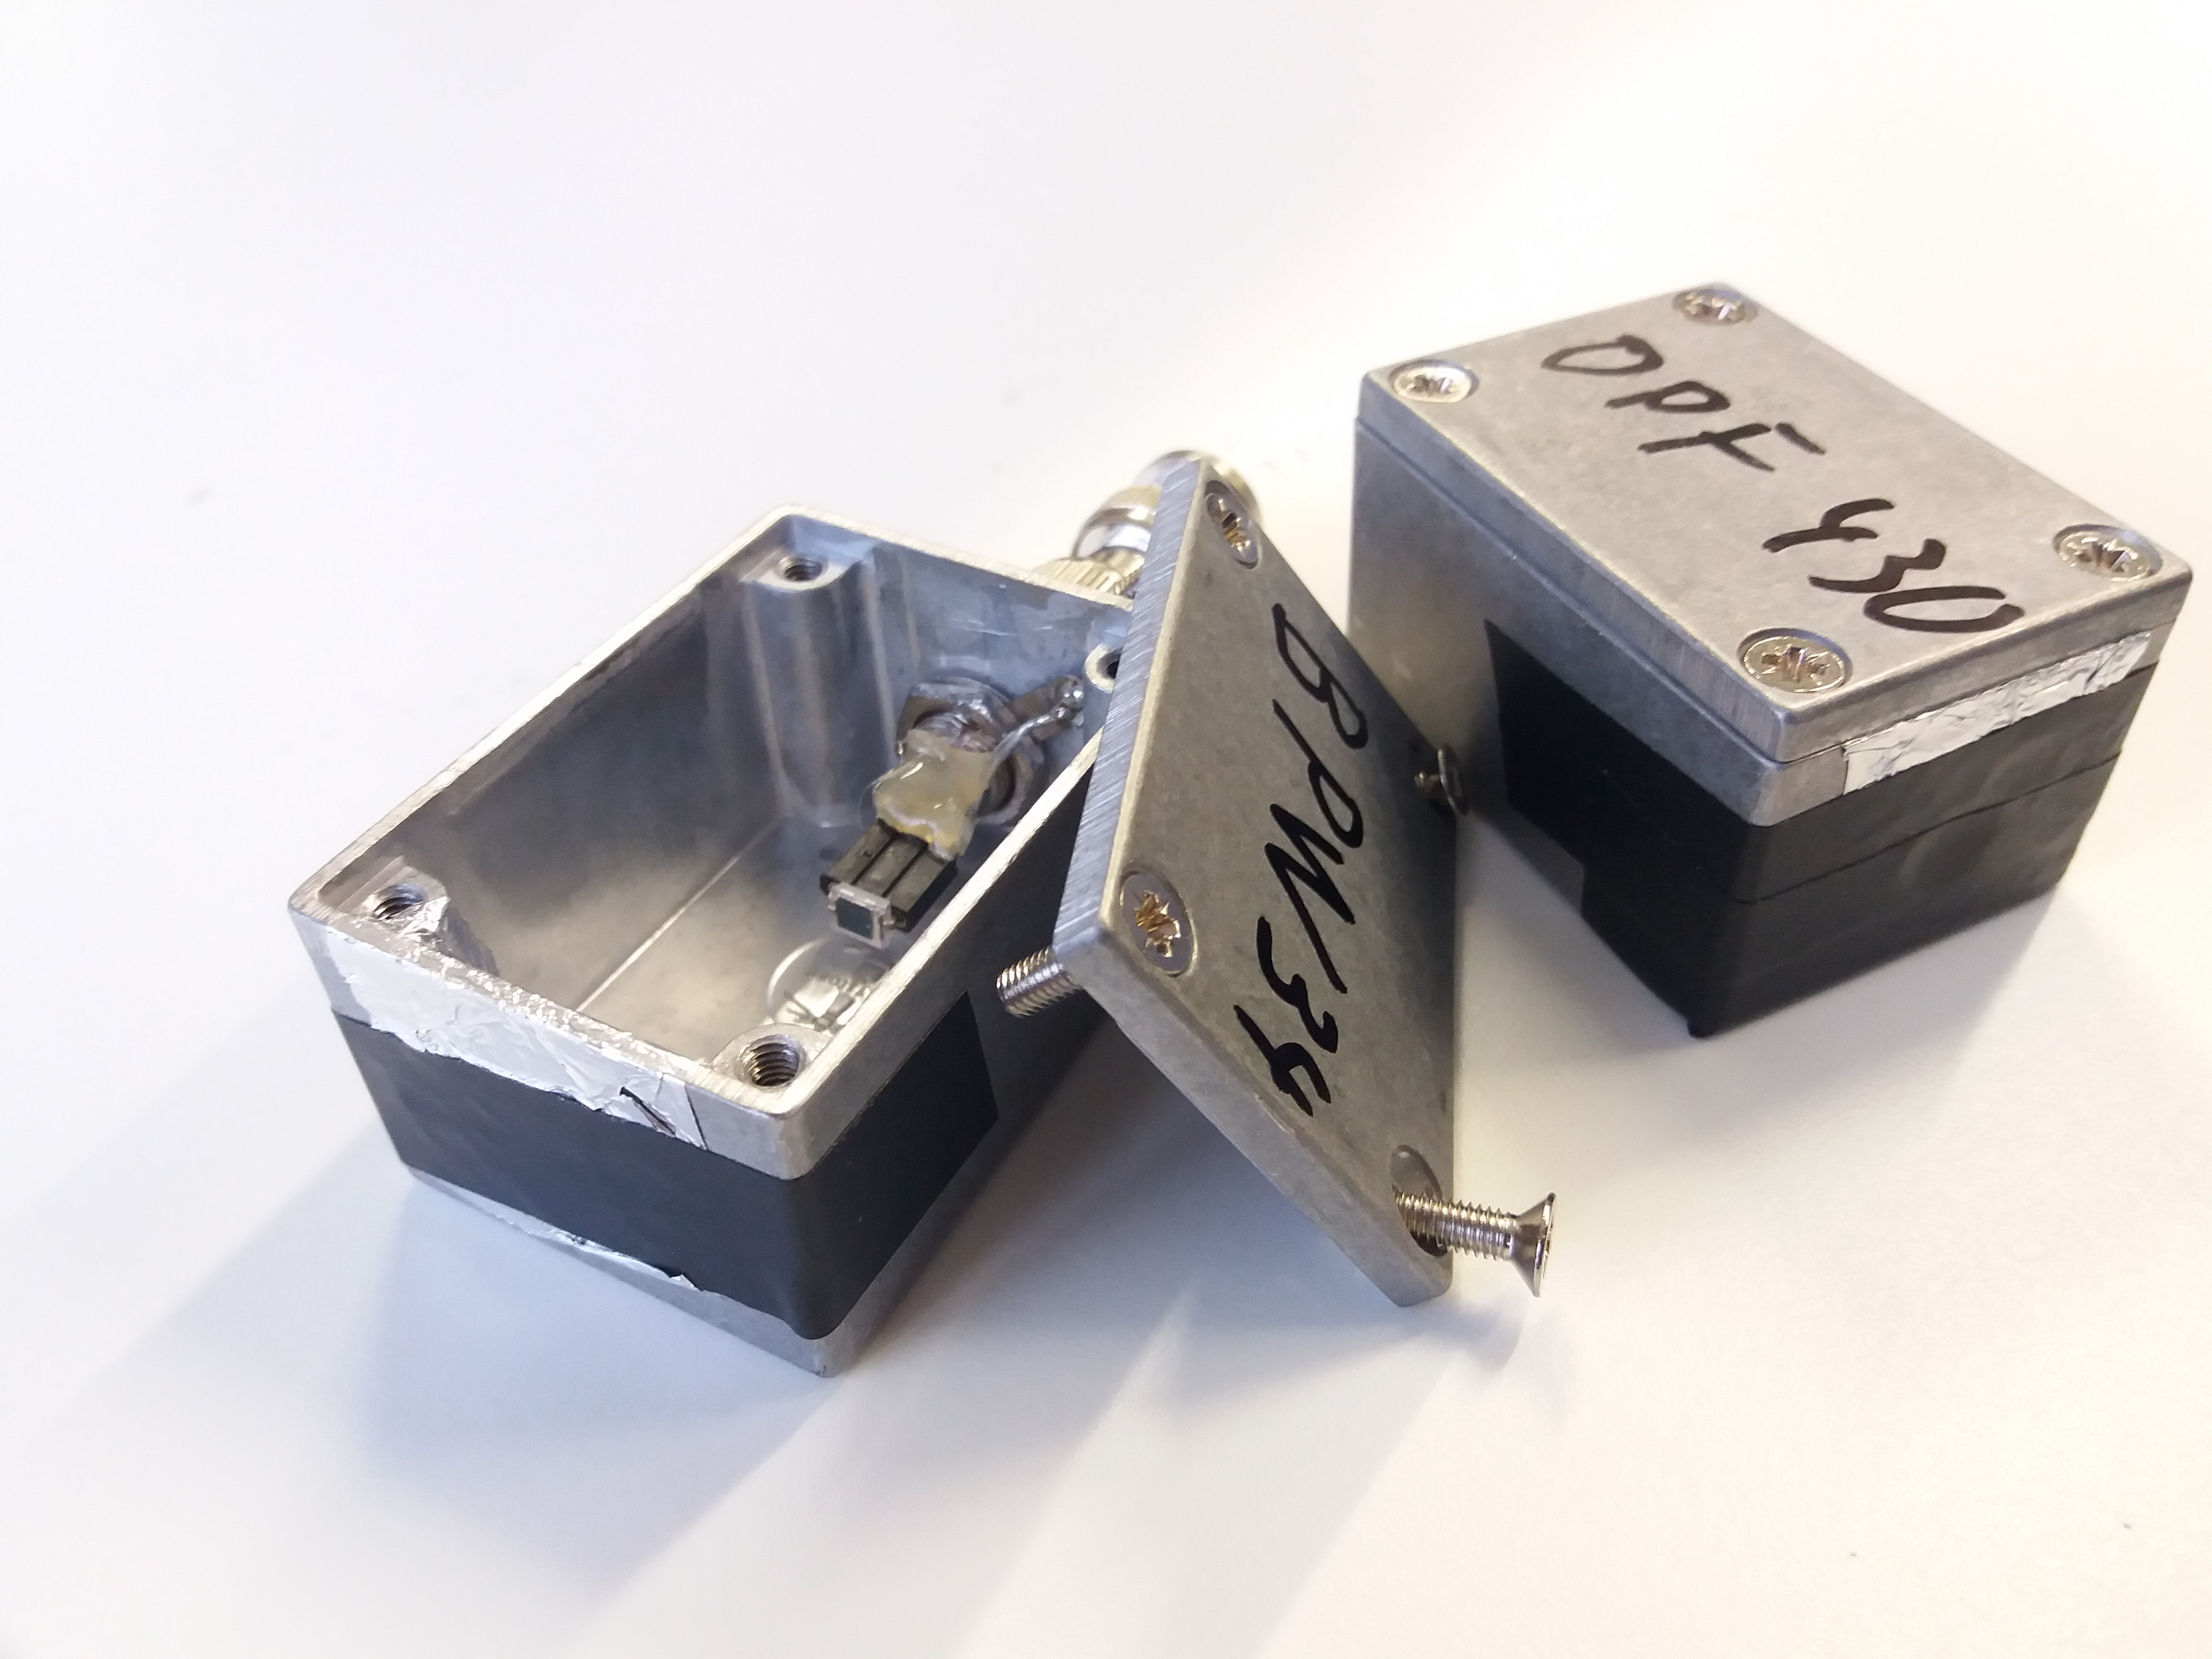
\includegraphics[scale=0.09, angle = 0]{./pictures/ShieldCrate.jpg}
 \caption{Photodiodes inside aluminium shielding crates.}
 \label{crate}
 
\end{figure}


%\begin{figure}[H]
% \centering
% 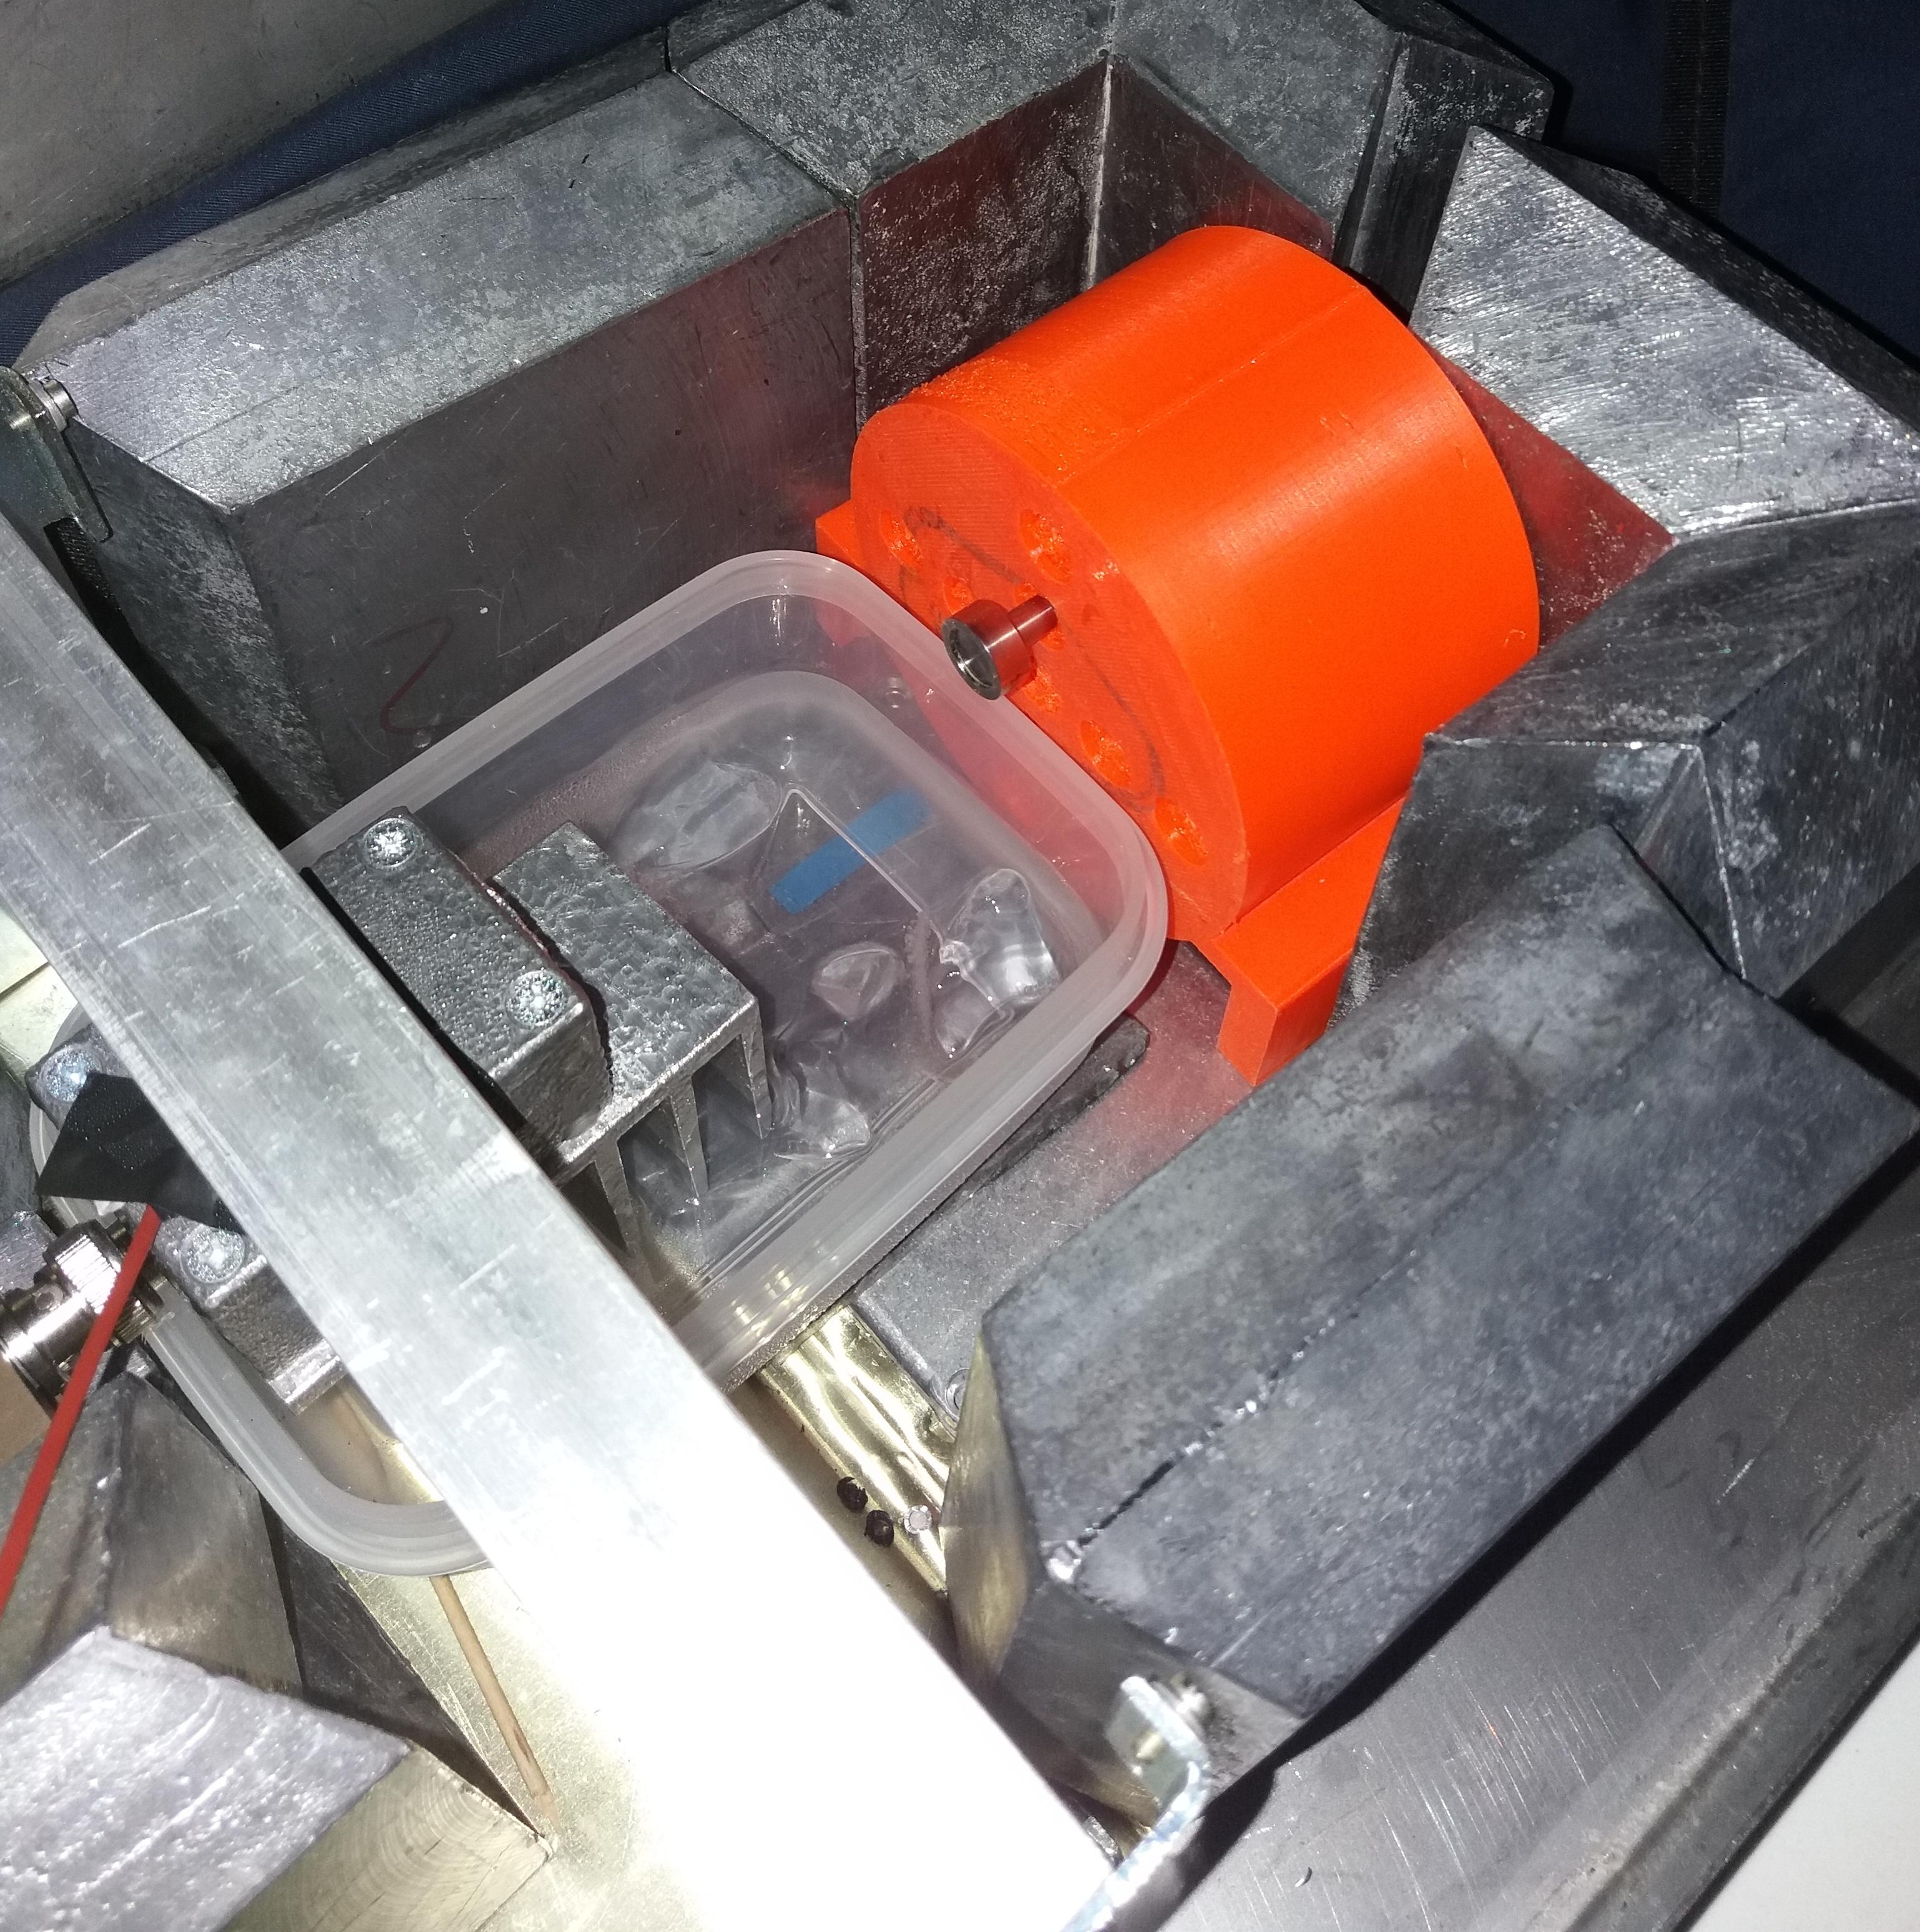
\includegraphics[scale=0.09, angle = 0]{./pictures/chlazeniLedem.jpg}
% \caption{Example of $^{57}$Co spectra from poorly shielded detector setup and from sufficiently shielded detector.}
% \label{notShielded}
% 
%\end{figure}





\subsection{Thermal noise reduction}
To reduce thermal noise, the S14605 photodiode was cooled with ice. It was placed in a shielding box with a heat sink attached to the bottom. This heat sink was submerged in the small tub filled with ice (see figure \ref{cooler}). Thermal conduction was improved by sticking the photodiode to the bottom of the shielding box with thermal paste. The photodiode was cooled in this way to temperatures around 7-8 $^\circ$C.
%To reduce the thermal noise, the S14605 photodiode was cooled by ice. It was placed in shielding box with attached heat sink to the bottom. This heat sink was submerged into the small tub filled with an ice (see Figure \ref{cooler}). The thermal conduction was improved by sticking the photodiode to the floor of the shielding box by a thermal paste. The photodiode was cooled this way to temperatures around 7-8 $^\circ$C.


\begin{figure}[H]
 \centering
 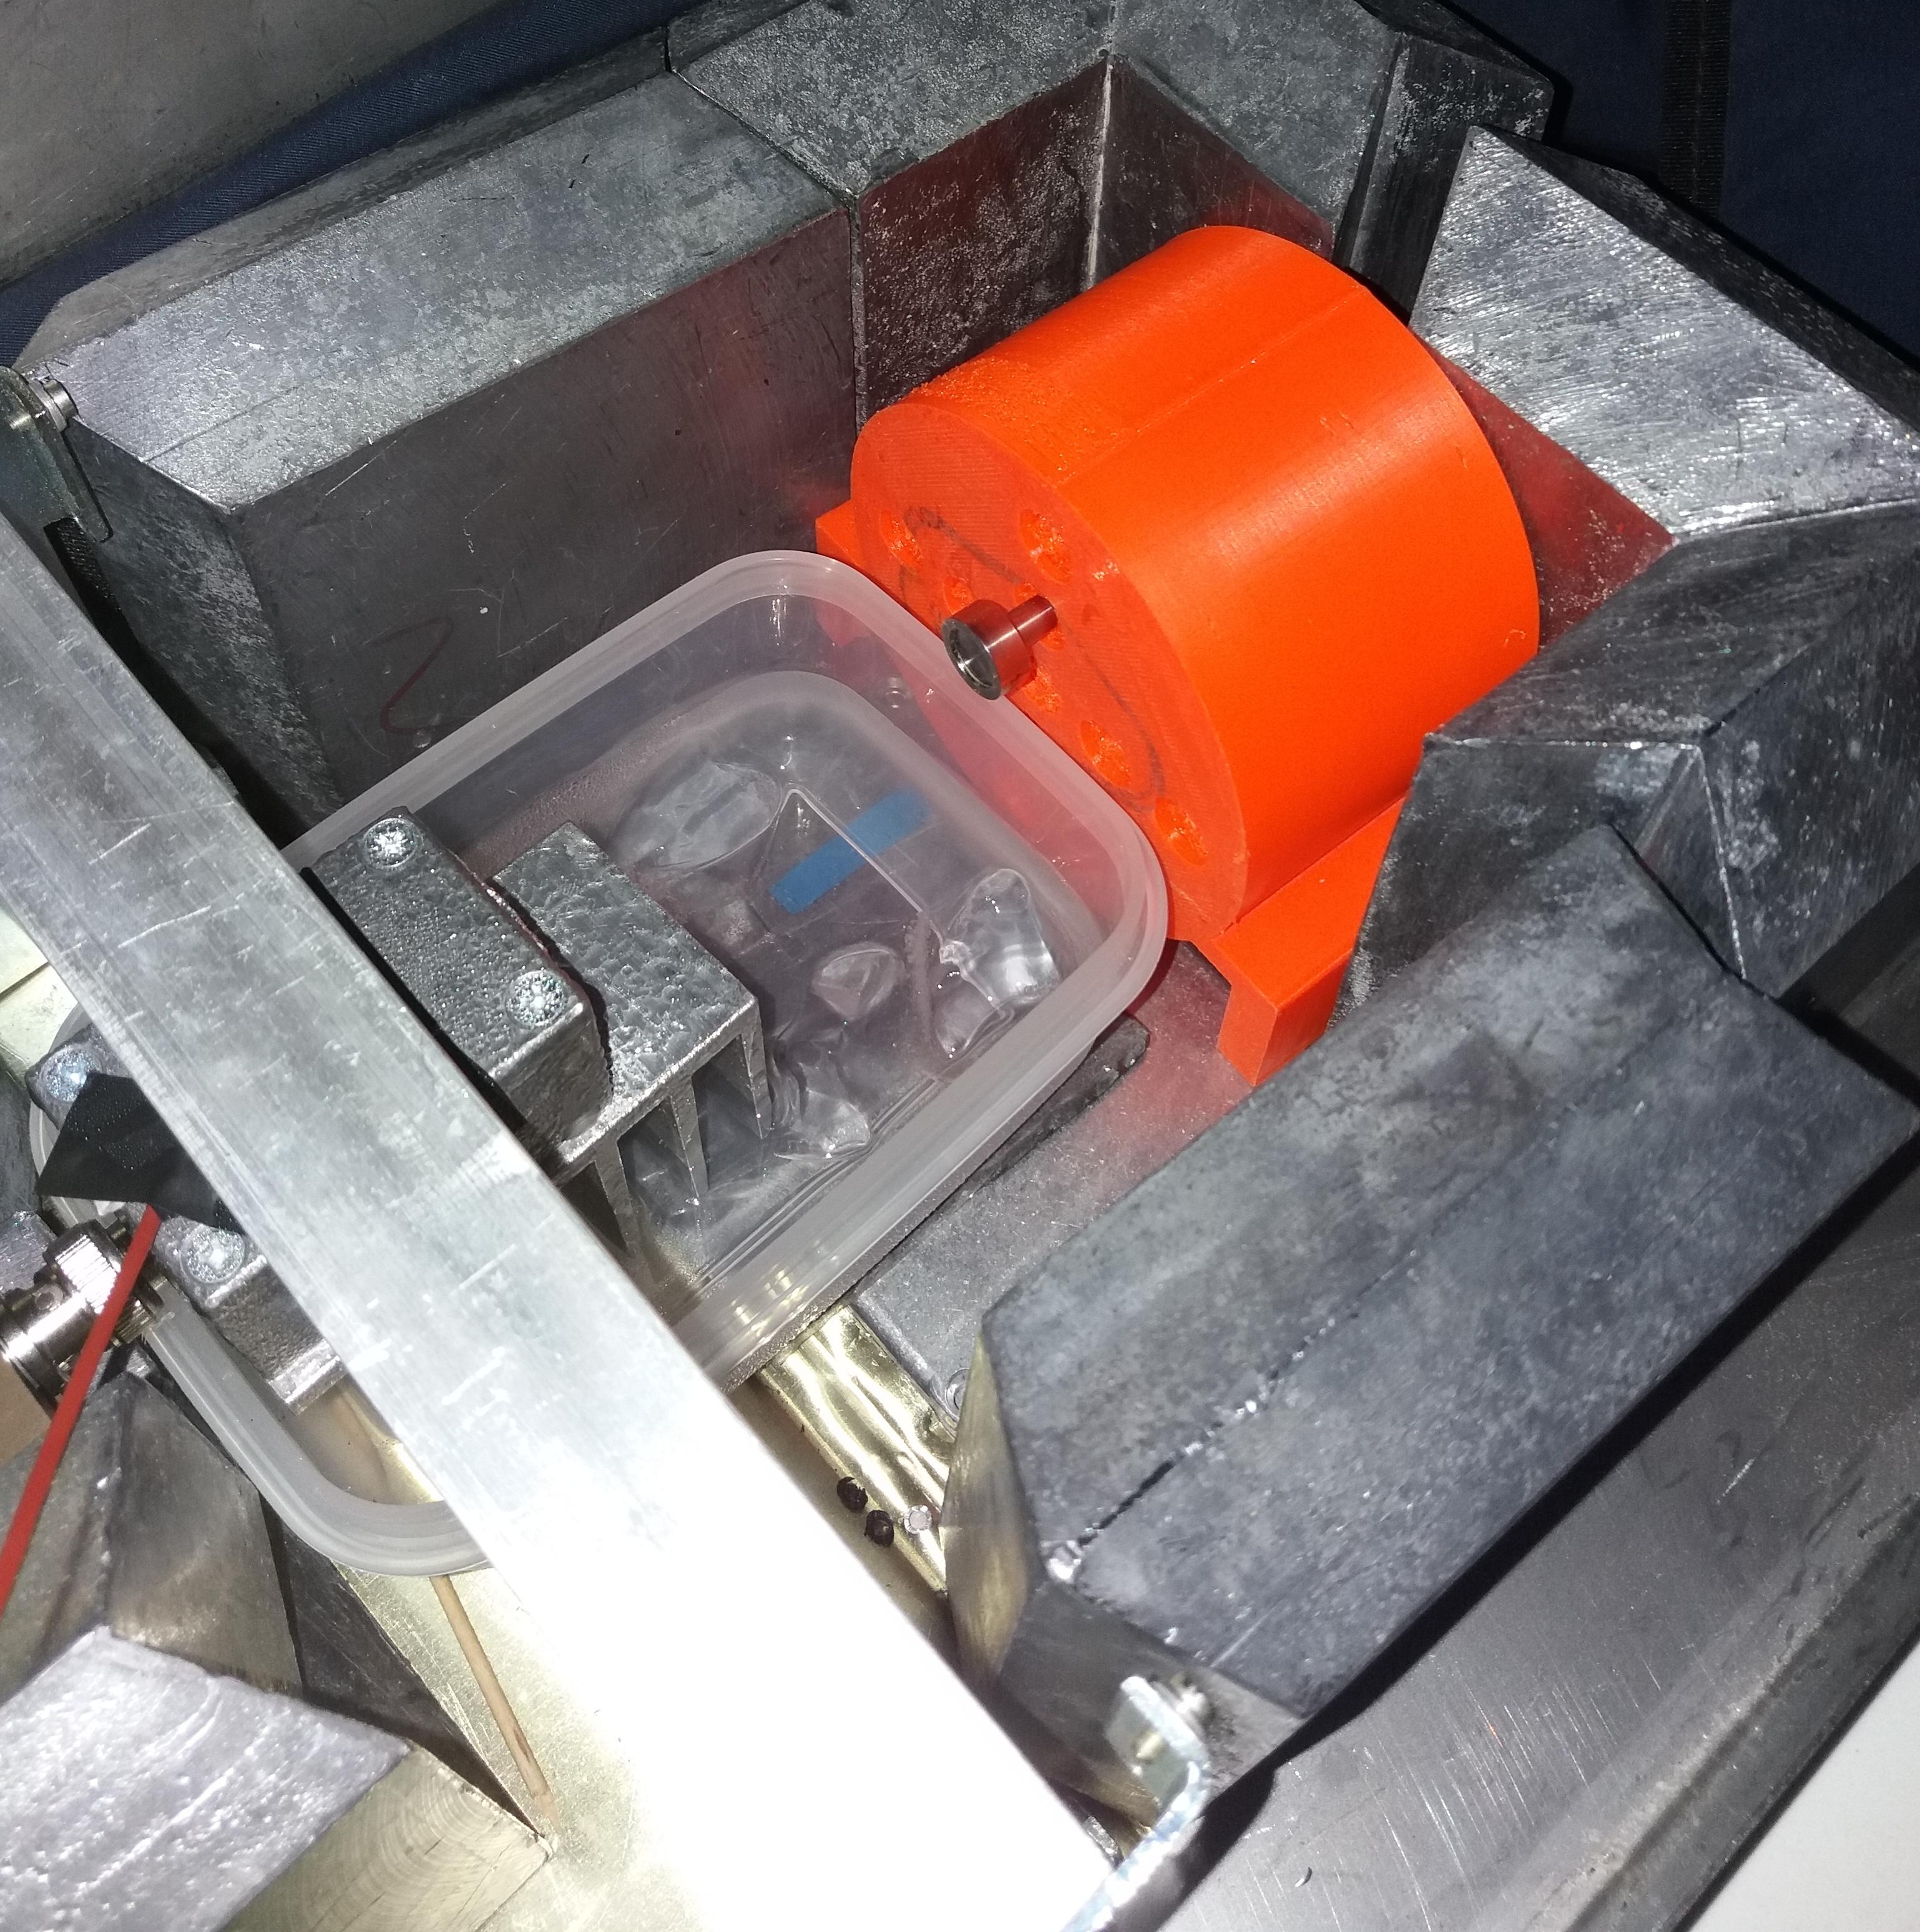
\includegraphics[scale=0.09, angle = 0]{./pictures/chlazeniLedem.png}
 \caption{Detector cooled by ice.}
 \label{cooler}
 
\end{figure}



\begin{figure}[H]
 \centering
 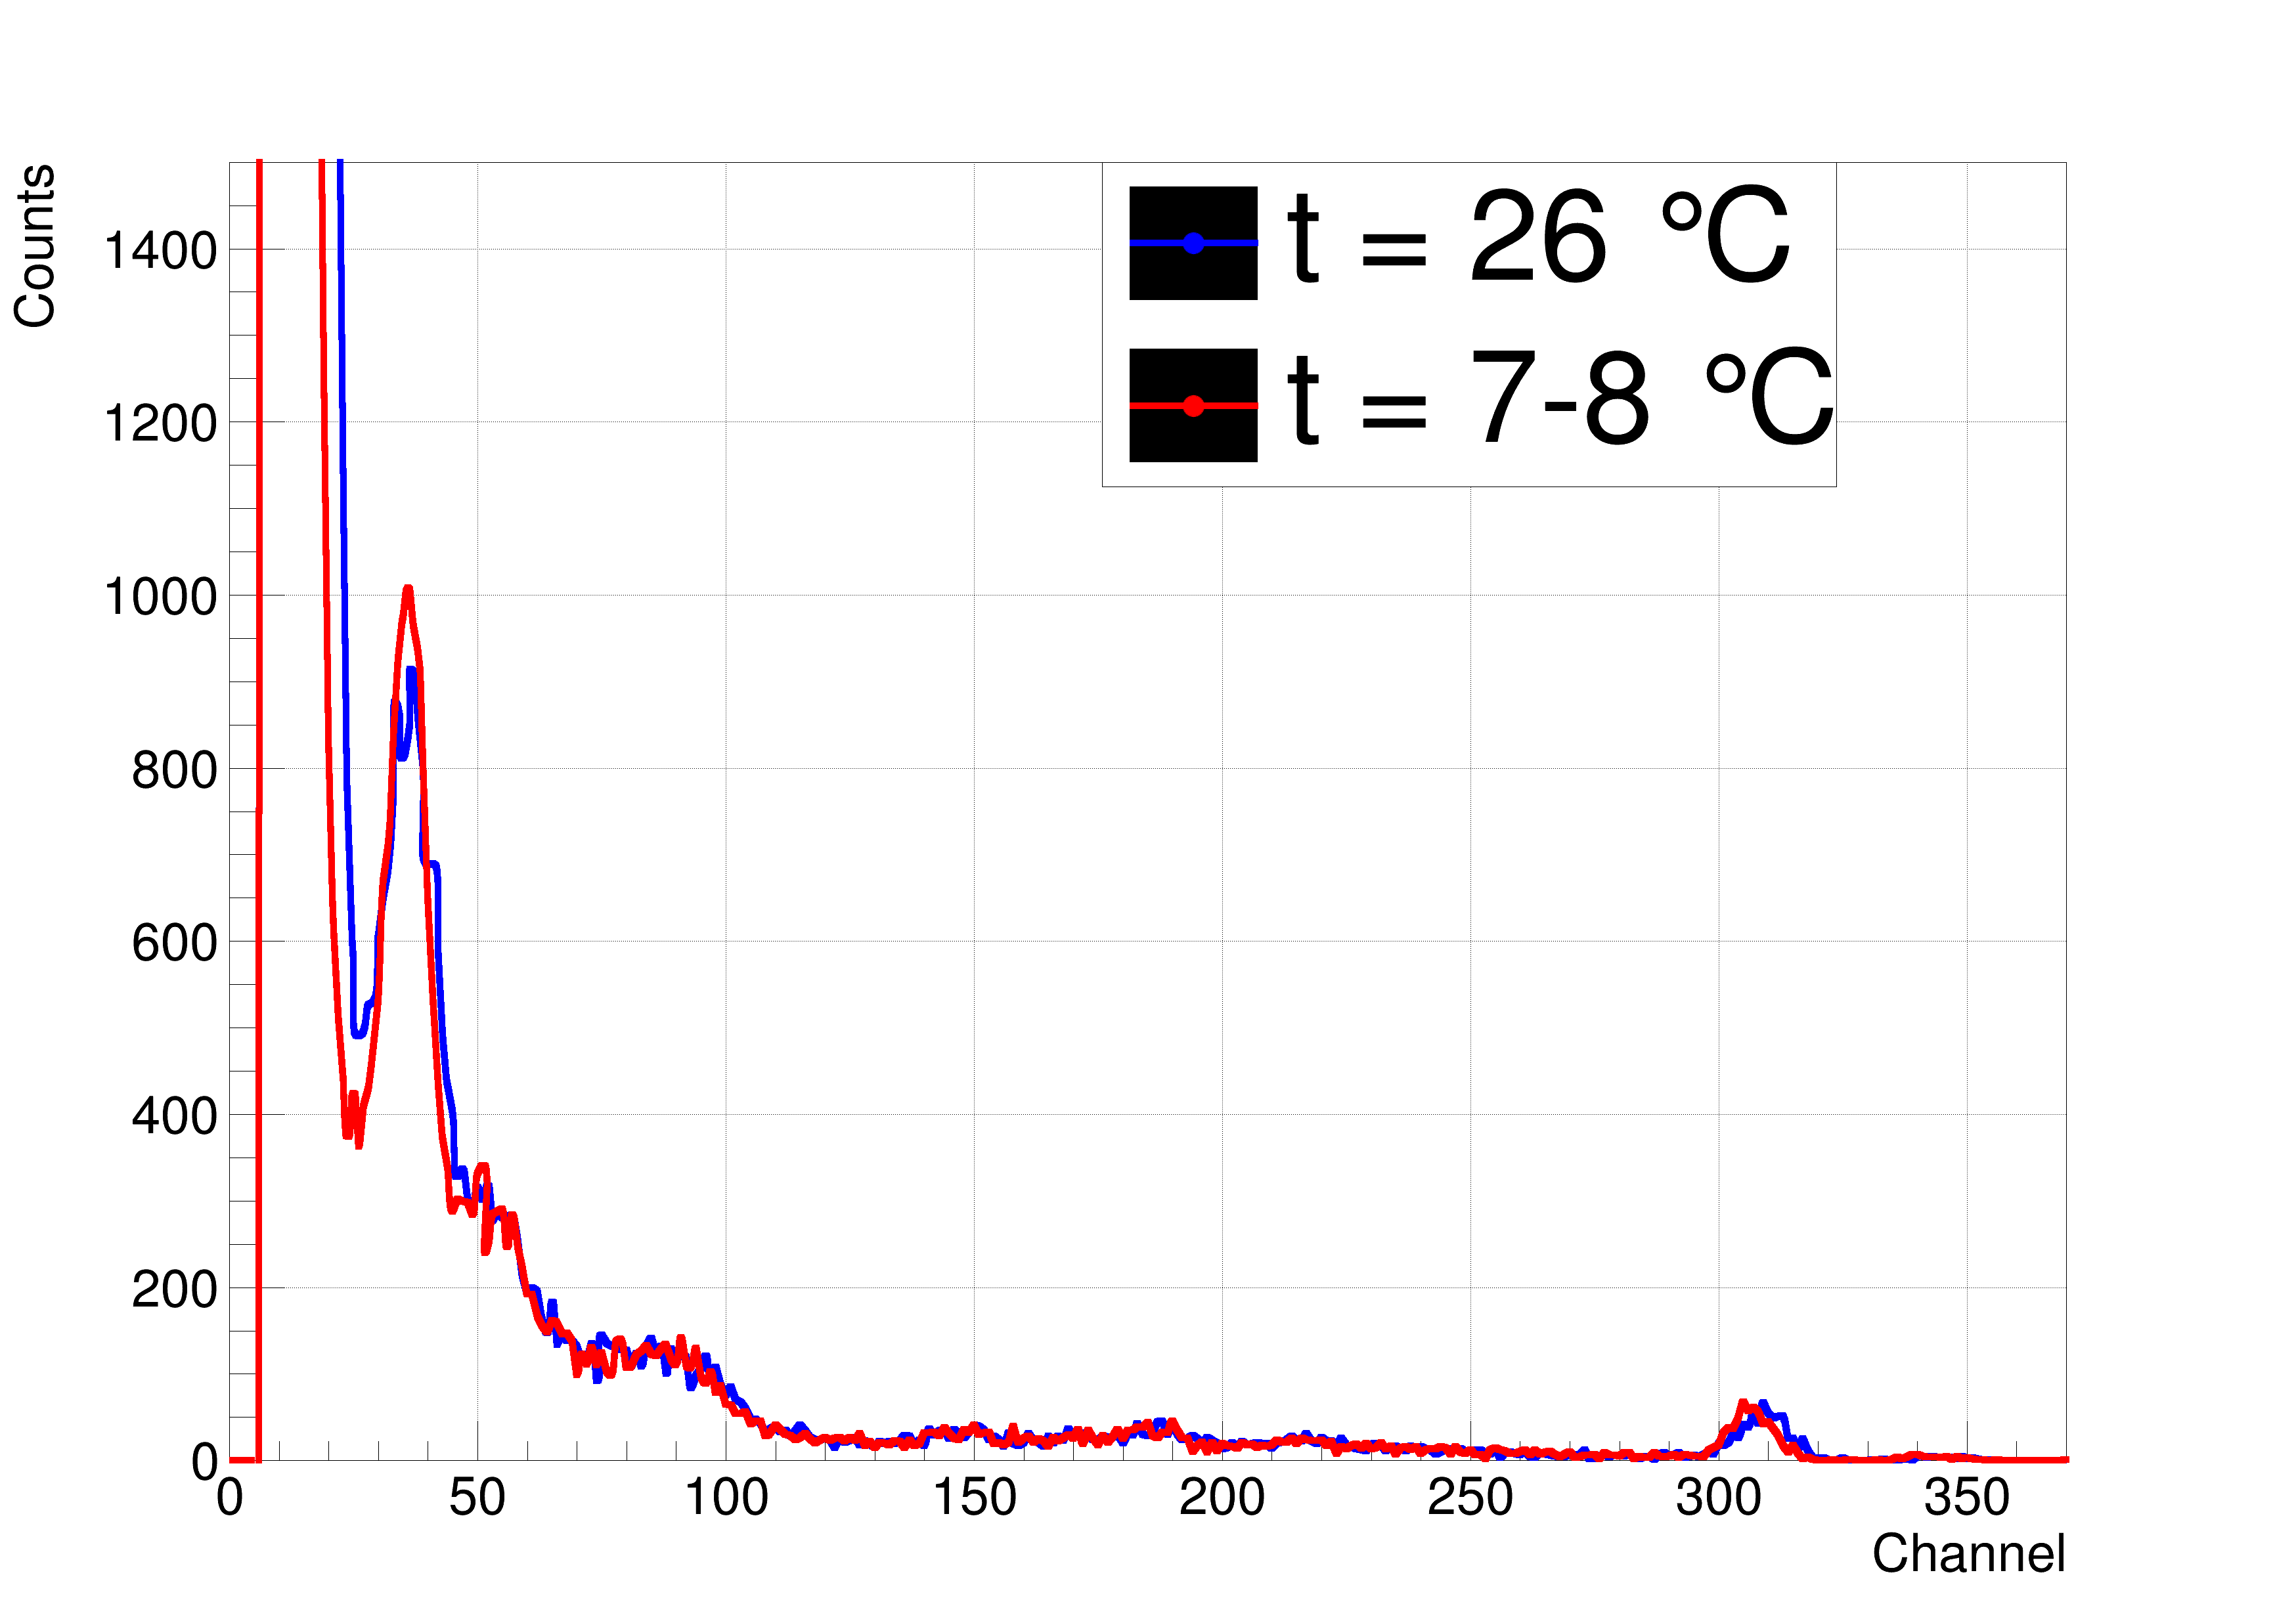
\includegraphics[scale=0.13, angle = 0]{./pictures/TempDiff.png}
 \caption{Measured $^{57}$Co spectra at two different temperatures.}
 \label{coolspectr}
 
\end{figure}
\par
The results show that cooling improves SNR, but its effect is small compared to the effect of proper shielding. The cooling is not used in the following tests on the ORTEC setup.


\section{Test measurement of the $^{57}$Co spectra}
The spectra for each photodiode were acquired for 30 min of live time - MCA allows dead time compensation which extends the total real time of the spectrum acquisition. The source was placed at a distance of 1 cm from the front shielding box (figure \ref{setup}) and to recognise the corresponding peaks, the set of the following filters was placed between the source and the detector:
%The spectra for each photodiode were taken for 30 min of live time - MCA allows dead time compensation, which extends the total real time of spectra acquisition. The source was placed into distance 1 cm from the front shielding crate (figure \ref{setup}) and to recognize the corresponding peaks, the set of the following filters were placed between source and detector:
\begin{itemize}
\item Pb filter: everything should be attenuated.
\item Cu filter: transmitted - 122.1 keV, 136.5 keV absorbed - 14.4 keV, 6.4 keV.
\item Al filter: transmitted - 122.1 keV, 136.5 keV, 14.4 keV absorbed - 6.4 keV.
\end{itemize}



\begin{figure}[H]
 \centering
 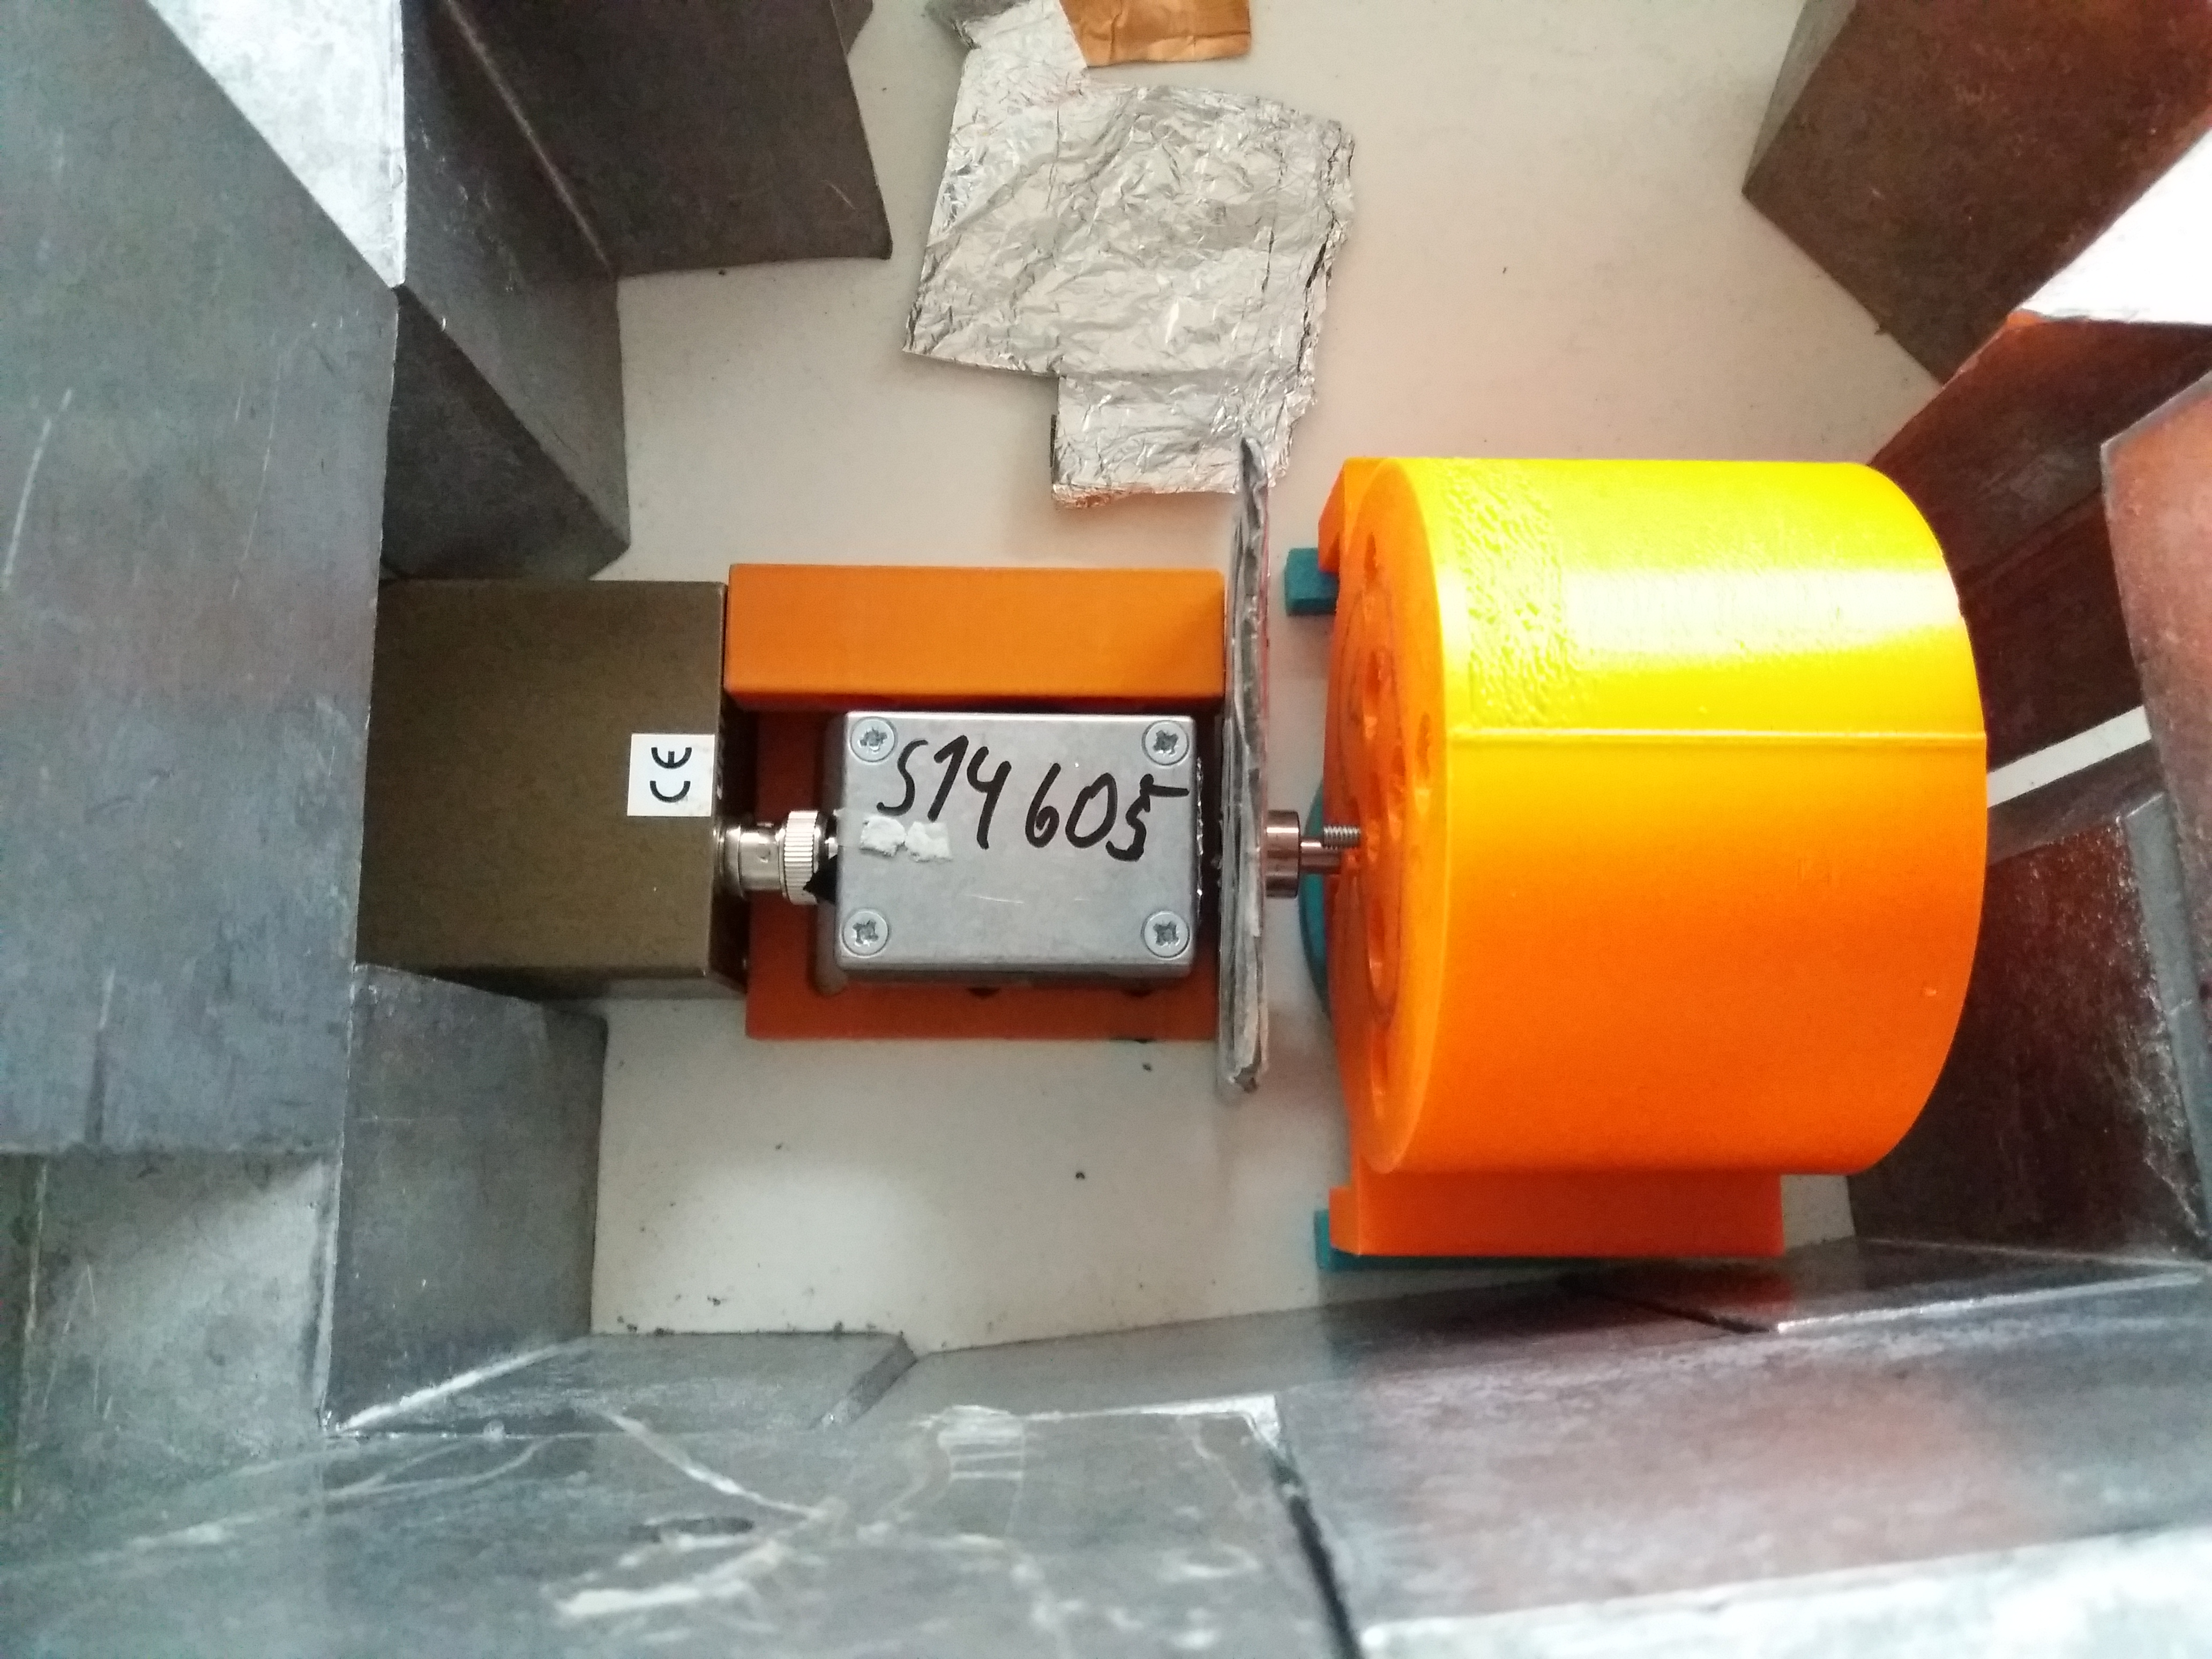
\includegraphics[scale=0.09, angle = 0]{./pictures/ORTECsetup.jpg}
 \caption{Setup for $^{57}$Co gamma spectrum measurement with filters. PIN photodiode  is situated inside the shielding crate, which is connected to the preamplifier.}
 \label{setup}
\end{figure}
The spectrum is analysed using our own peak finder program (described in section \ref{search}) to find the characteristic energy components. The 14.4 keV channel position is then used to calibrate the energy axis of the MCA spectrum. The Compton edge caused by the interaction of 122.1 keV photons inside the detector can be expected. The equation \ref{compton} predicts the position to be around 39.5 keV.
%The spectrum is analysed by our own peak finder program (described in section \ref{search}) to find the characteristic energy components. The channel position of 14.4 keV is then used to to calibrate the energy axis of the MCA spectrum. The Compton edge caused by interaction of 122.1 keV photons inside the detector can be expected. The equation \ref{compton} predicts the position to be around 39.5 keV.
\subsection{S14605 test}
The optimal bias voltage of 50 V has been determined experimentally - any further increase does not improve the noise. The measured spectra with no filter, with special filters and only background (fully shielded) are shown in the figure \ref{S14605 spectra}.
%The optimal bias voltage 50 V was deduced experimentally - any further increase does not improve the noise. The measured spectra with no filter, with particular filters and only background (fully shielded) are in the figure \ref{S14605 spectra}.


\begin{figure}[H]
 \centering
 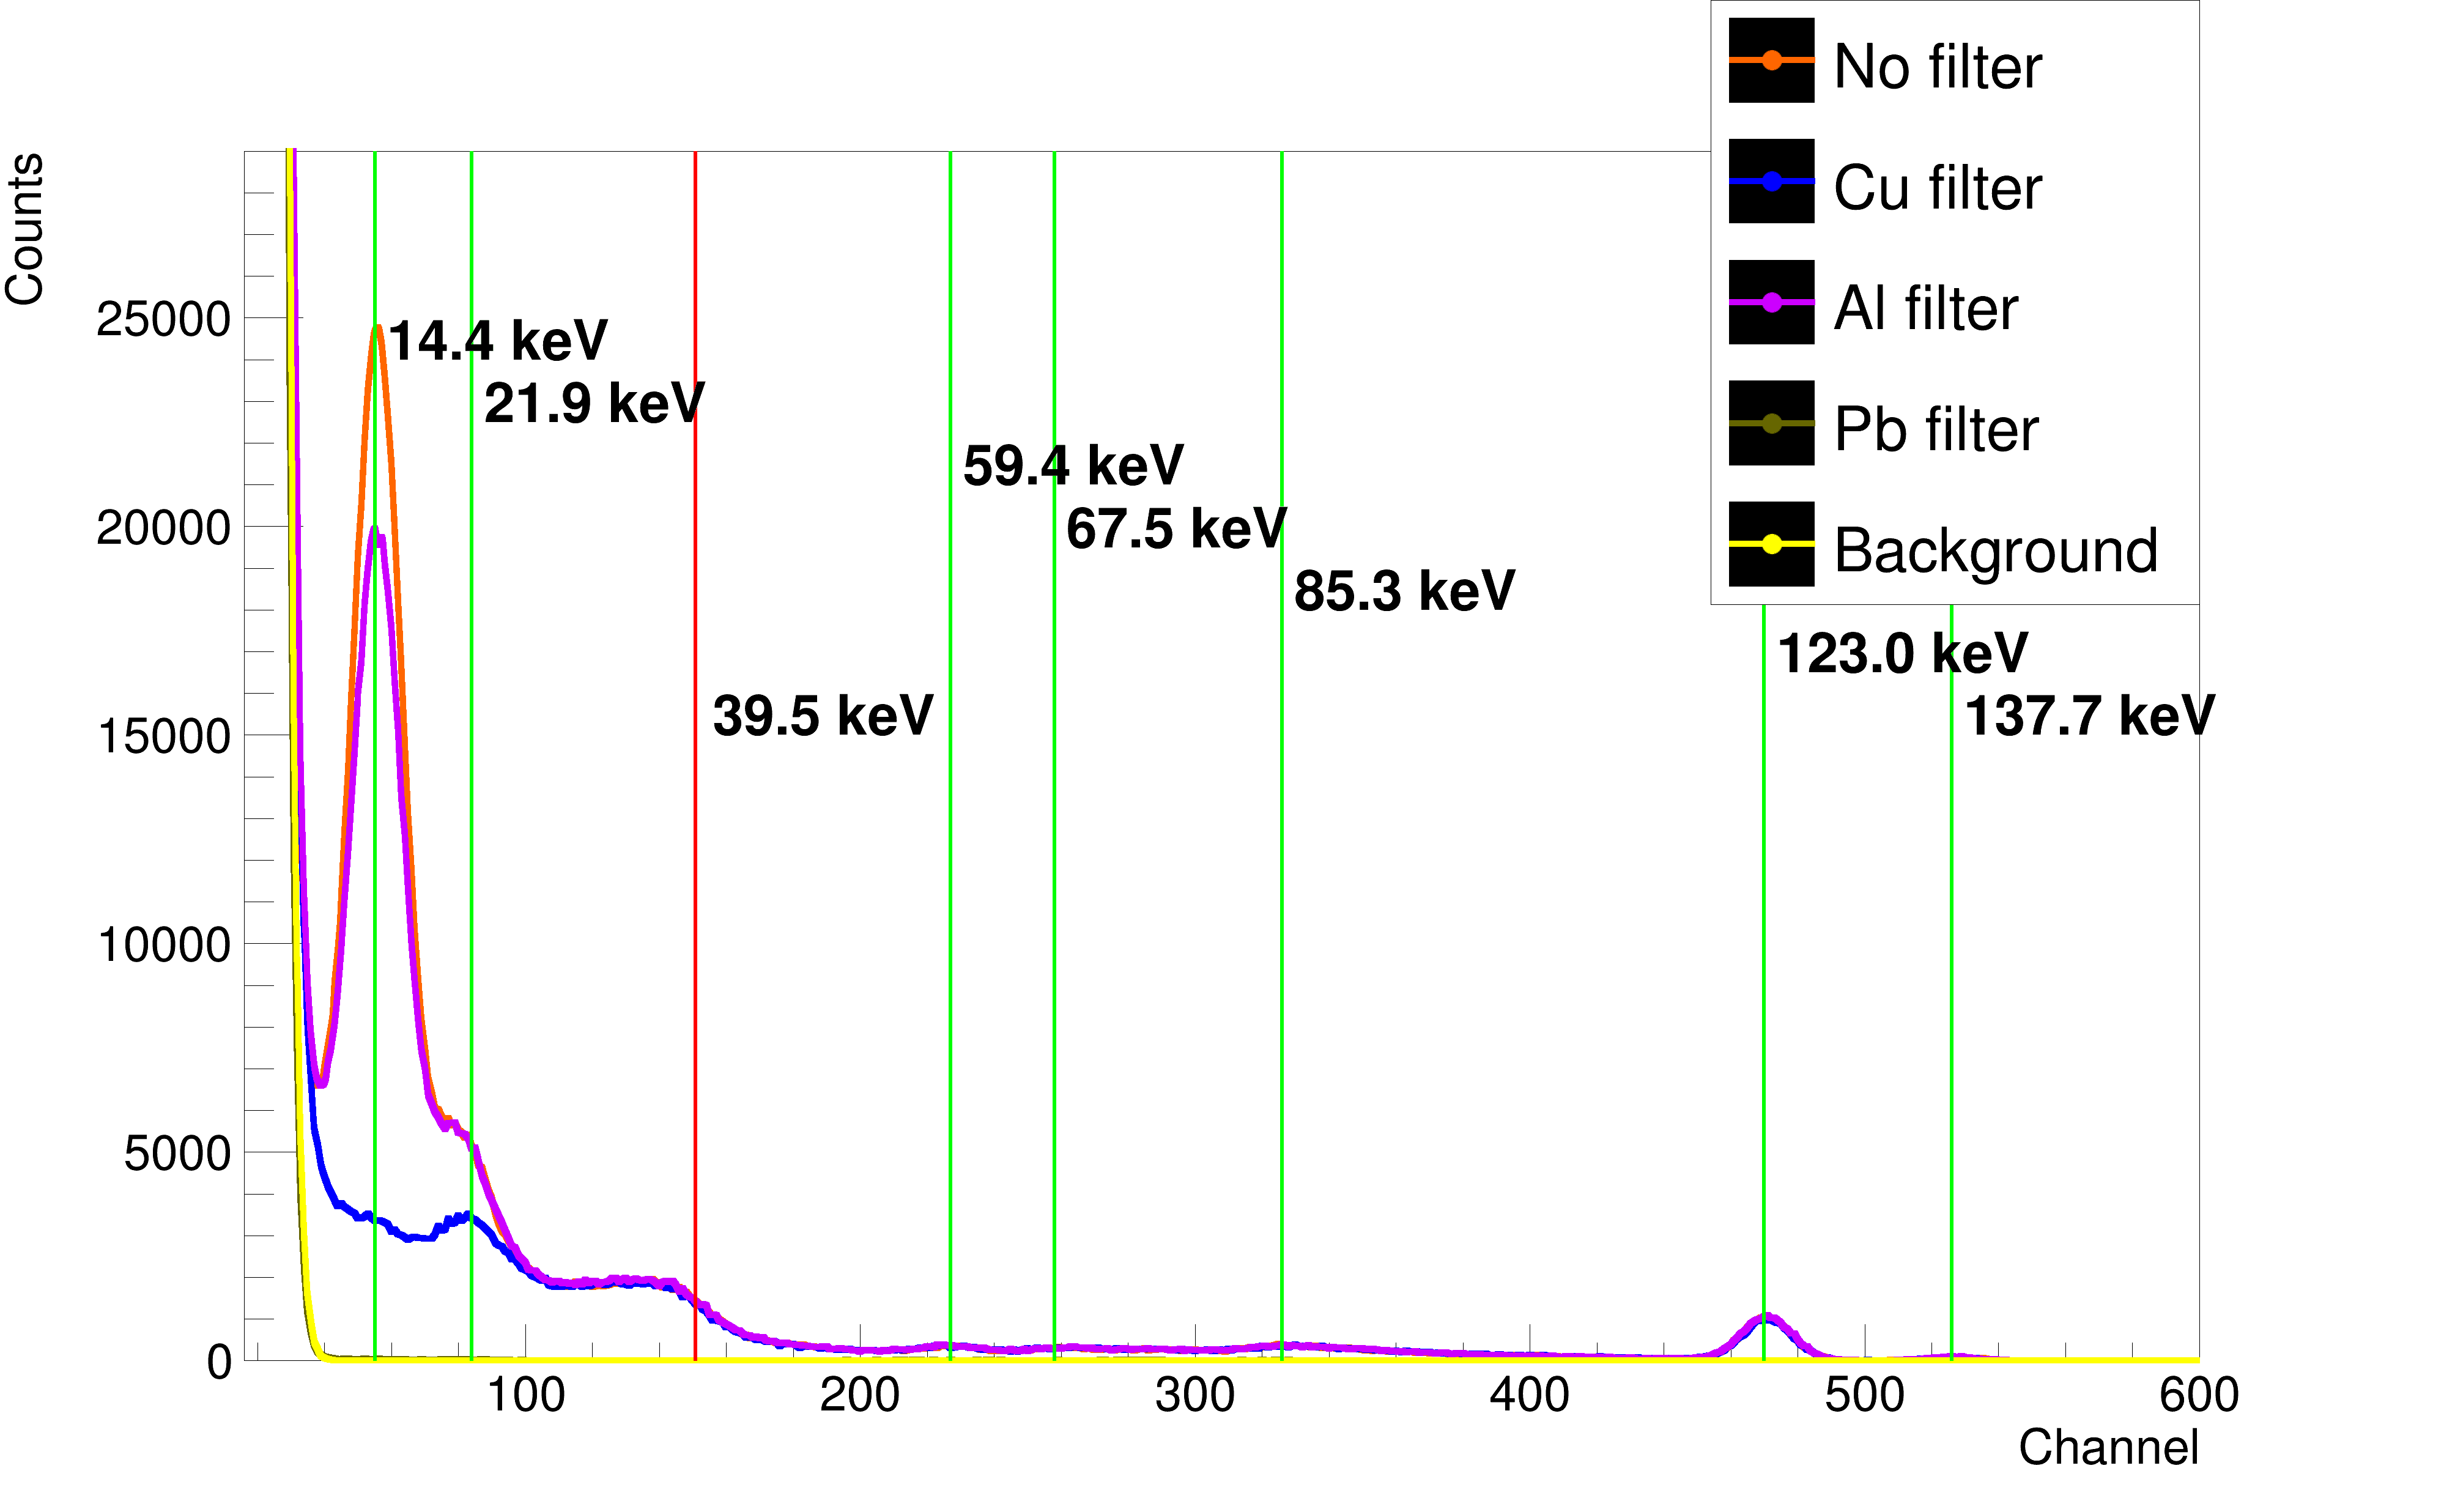
\includegraphics[scale=0.125, angle = 0]{./pictures/S14GammaTest.png}
 \caption{S14605 spectra with founded energy peaks (green lines) and predicted Compton edge (red line).}
 \label{S14605 spectra}
 
\end{figure}


\par
The first peak was determined to be a 14.4 full energy peak as it is absorbed by the Cu filter. The 21.9 keV peak is from characteristic X-rays of the rhodium matrix, and 59.4 keV may also originate from the source matrix. The 67.5 keV and 85.3 keV peaks are most likely characteristic X-rays from the lead shielding. The last two peaks (123.0 keV, 137.7 keV) are from $^{57}$Co. It can be seen that the detection efficiency of the full energy at higher energies (122.1 keV) is very low, and that Compton scattering is preferred interaction effect inside the detector at these energies, resulting in the expected Compton edge. The expected peak at 6.4 keV is hidden in the electronic noise.
%The first peak was determined as 14.4 full energy peak, because the Cu filter absorbs it. The 21.9 keV peak originates from characteristic x-rays of rhodium matrice and 59.4 keV also possibly originates from the source matrice. The 67.5 keV 85.3 keV peaks are most probably characteristic x-ray photons of lead shielding. The last two peaks (123.0 keV, 137.7 keV) are from $^{57}$Co. It can be seen that the full energy detection efficiency of higher energies (122.1 keV) is very small and that the Compton scattering is preferred interaction effect inside detector at these energies, which results into expected Compton edge. The expected peak of 6.4 keV is hidden in the electronic noise.

\subsection{BPW34 test}
The instrumentation was similar to before, but BPW34 had to be operated at a lower bias voltage, so 20 V was chosen as the optimum. The measured spectra are shown in the figure \ref{BPW34 spectra}.
%The instrumentation was similar as before, but BPW34 had to be operated at lower bias voltage and thus 20 V was chosen as an optimum. Measured spectra are in the figure \ref{BPW34 spectra}.

\begin{figure}[H]
 \centering
 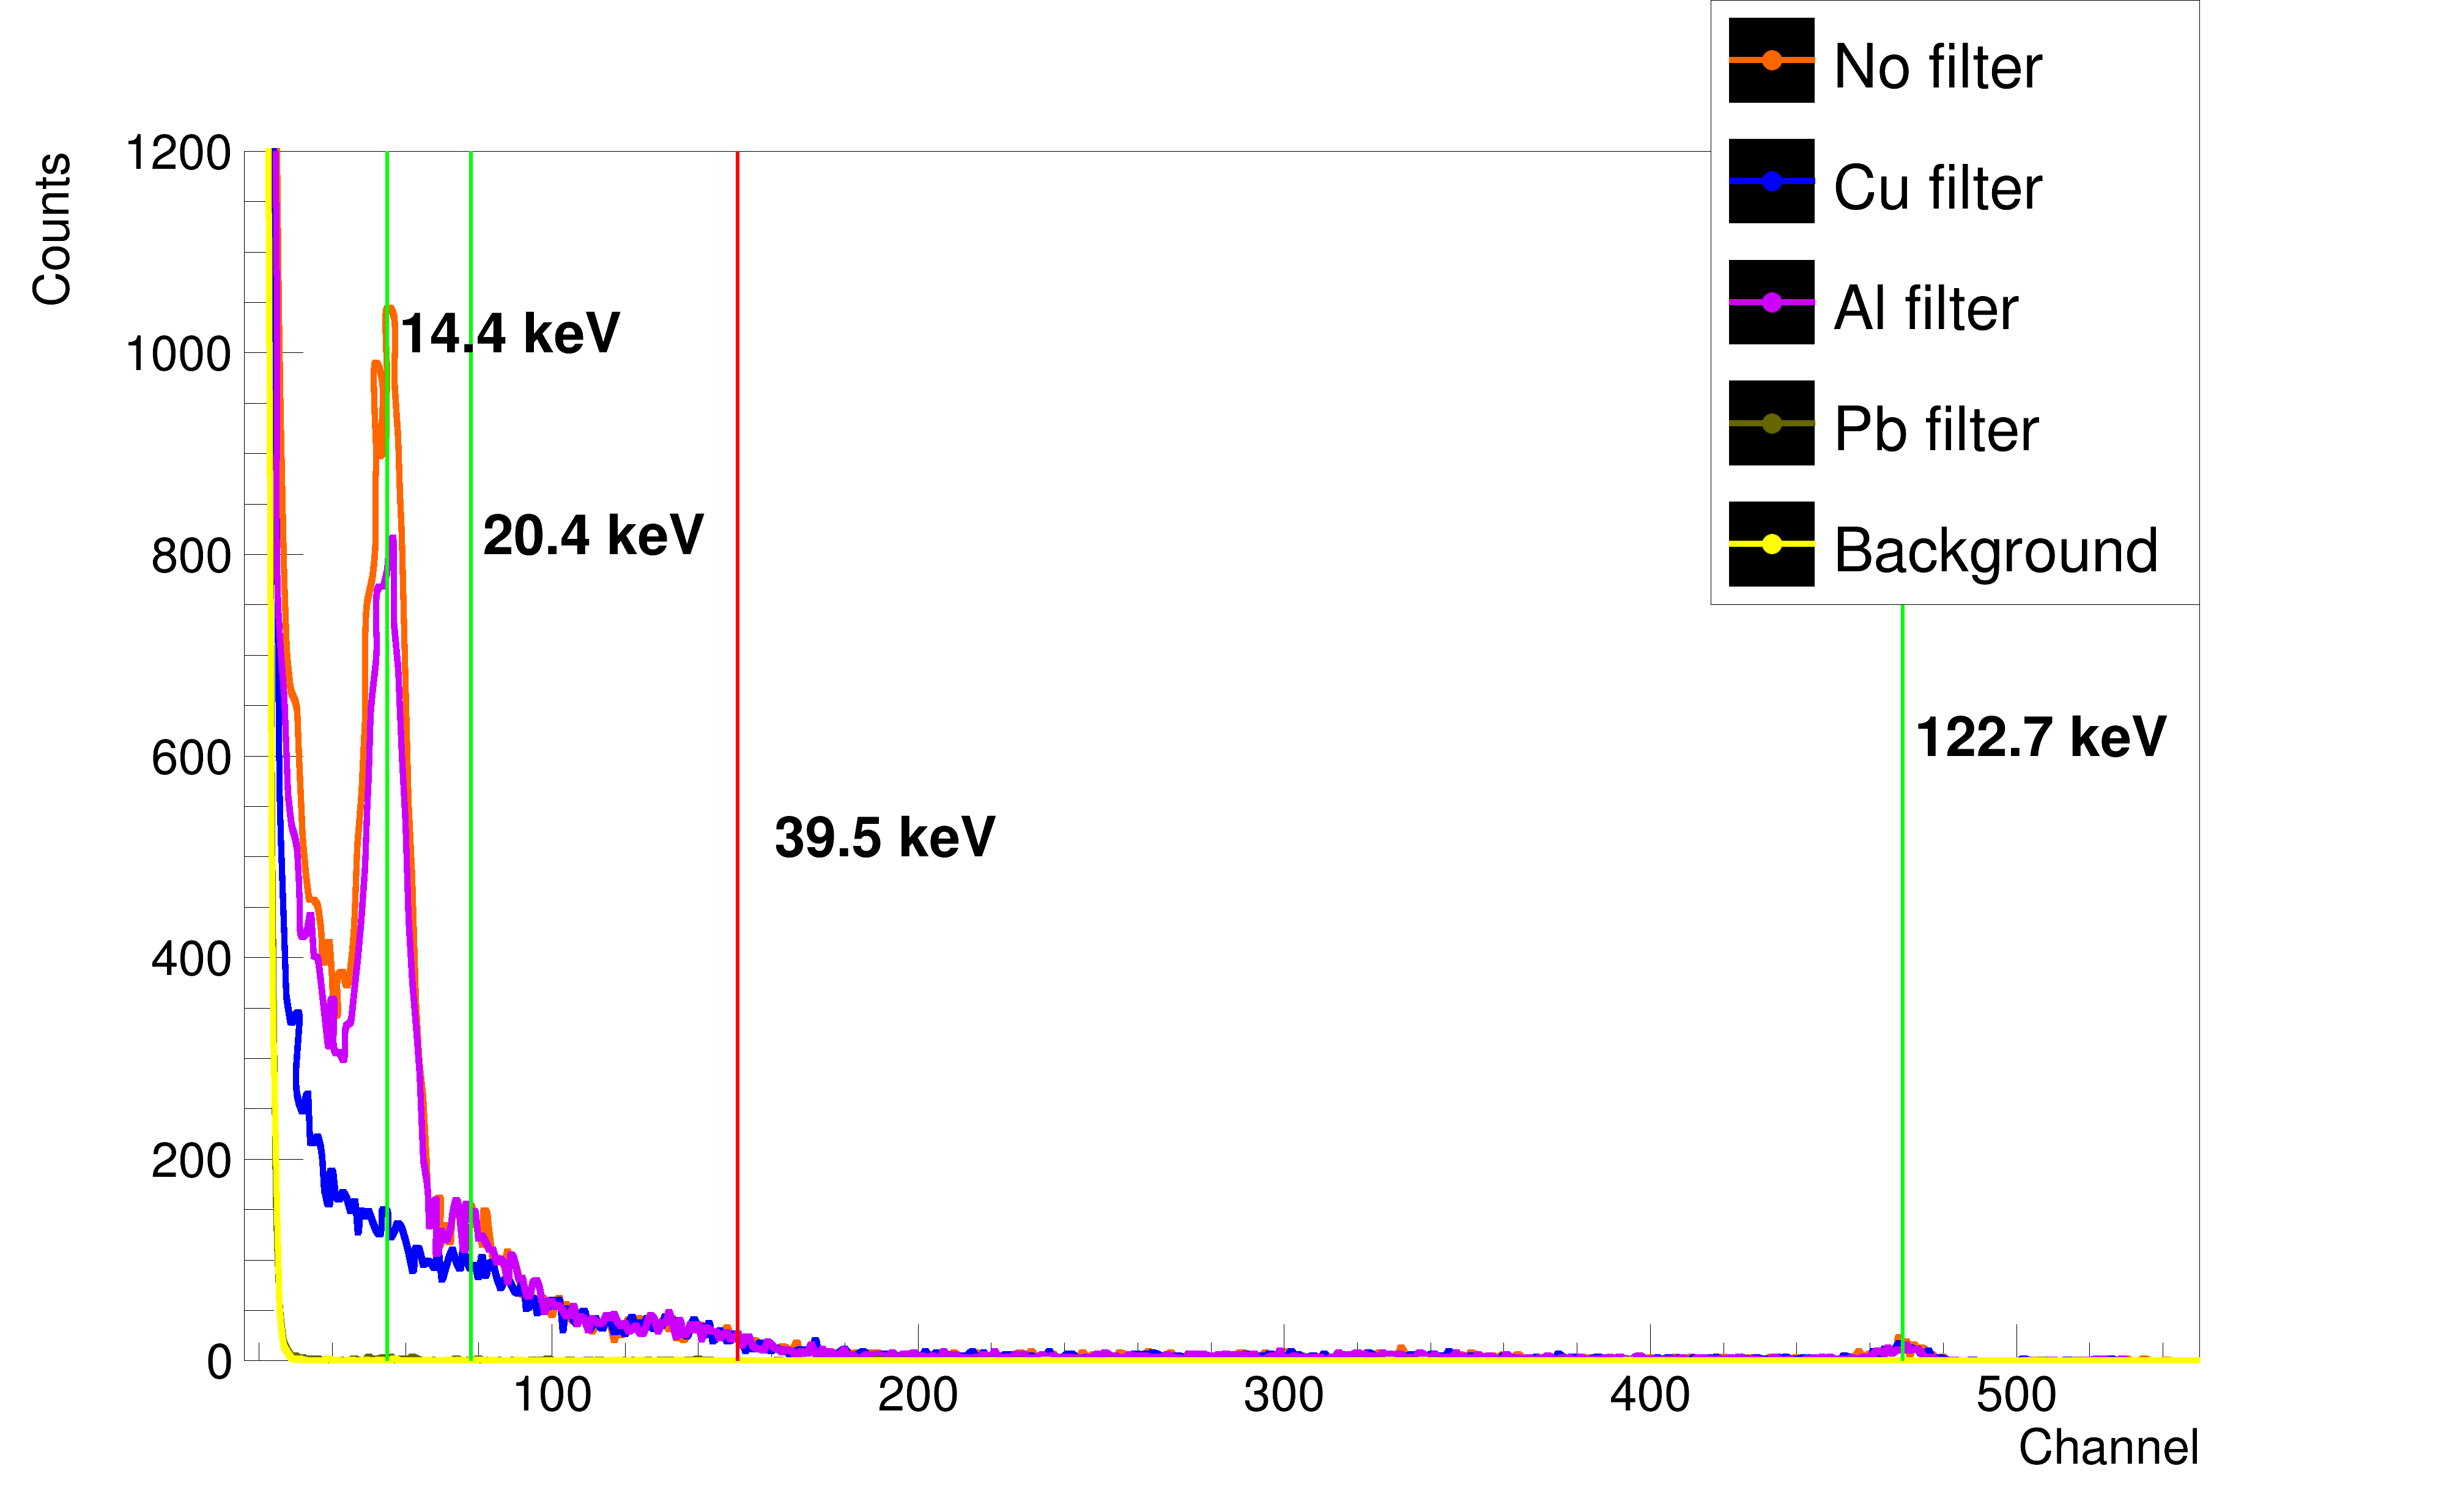
\includegraphics[scale=0.125, angle = 0]{./pictures/BPW34GammaTest.png}
  \caption{BPW34 spectra with founded energy peaks (green lines) and predicted Compton edge (red line).}
 \label{BPW34 spectra}
 
\end{figure}
The measured spectra of BPW34 are very similar to the previous one, but the peak heights are about 25 times lower. The results also confirm the fact that the Si semiconductor structure with p-n or p-i-n junction detects the gamma photons with the same signal strength without any dependence on the dimensions. Only the detection efficiency depends on the dimensions.
%The measured spectra of BPW34 is very similar to the previous one, however the peak's heights are approximately 25 times lower. The results also confirm the fact that the Si semiconductor structure with p-n or p-i-n junction detects the gamma photons with the same signal strength without any dependency on the dimensions. Only the detection efficiency is dependent on the dimensions.
\subsection{OPF430 test}
The OPF430 was operated at 20 V. There was a problem with the very low detection efficiency, so the source had to be placed in the shielding box just before the photodiode. Spectra acquired in this way are shown in the figure \ref{OPF430 spectra}.
%OPF430 was operated at 20 V. There was a problem with the very low detection efficiency, so the source had to be put into the shielding box right before the photodiode. Spectra acquired this way are in the figure \ref{OPF430 spectra}.

\begin{figure}[H]
 \centering
 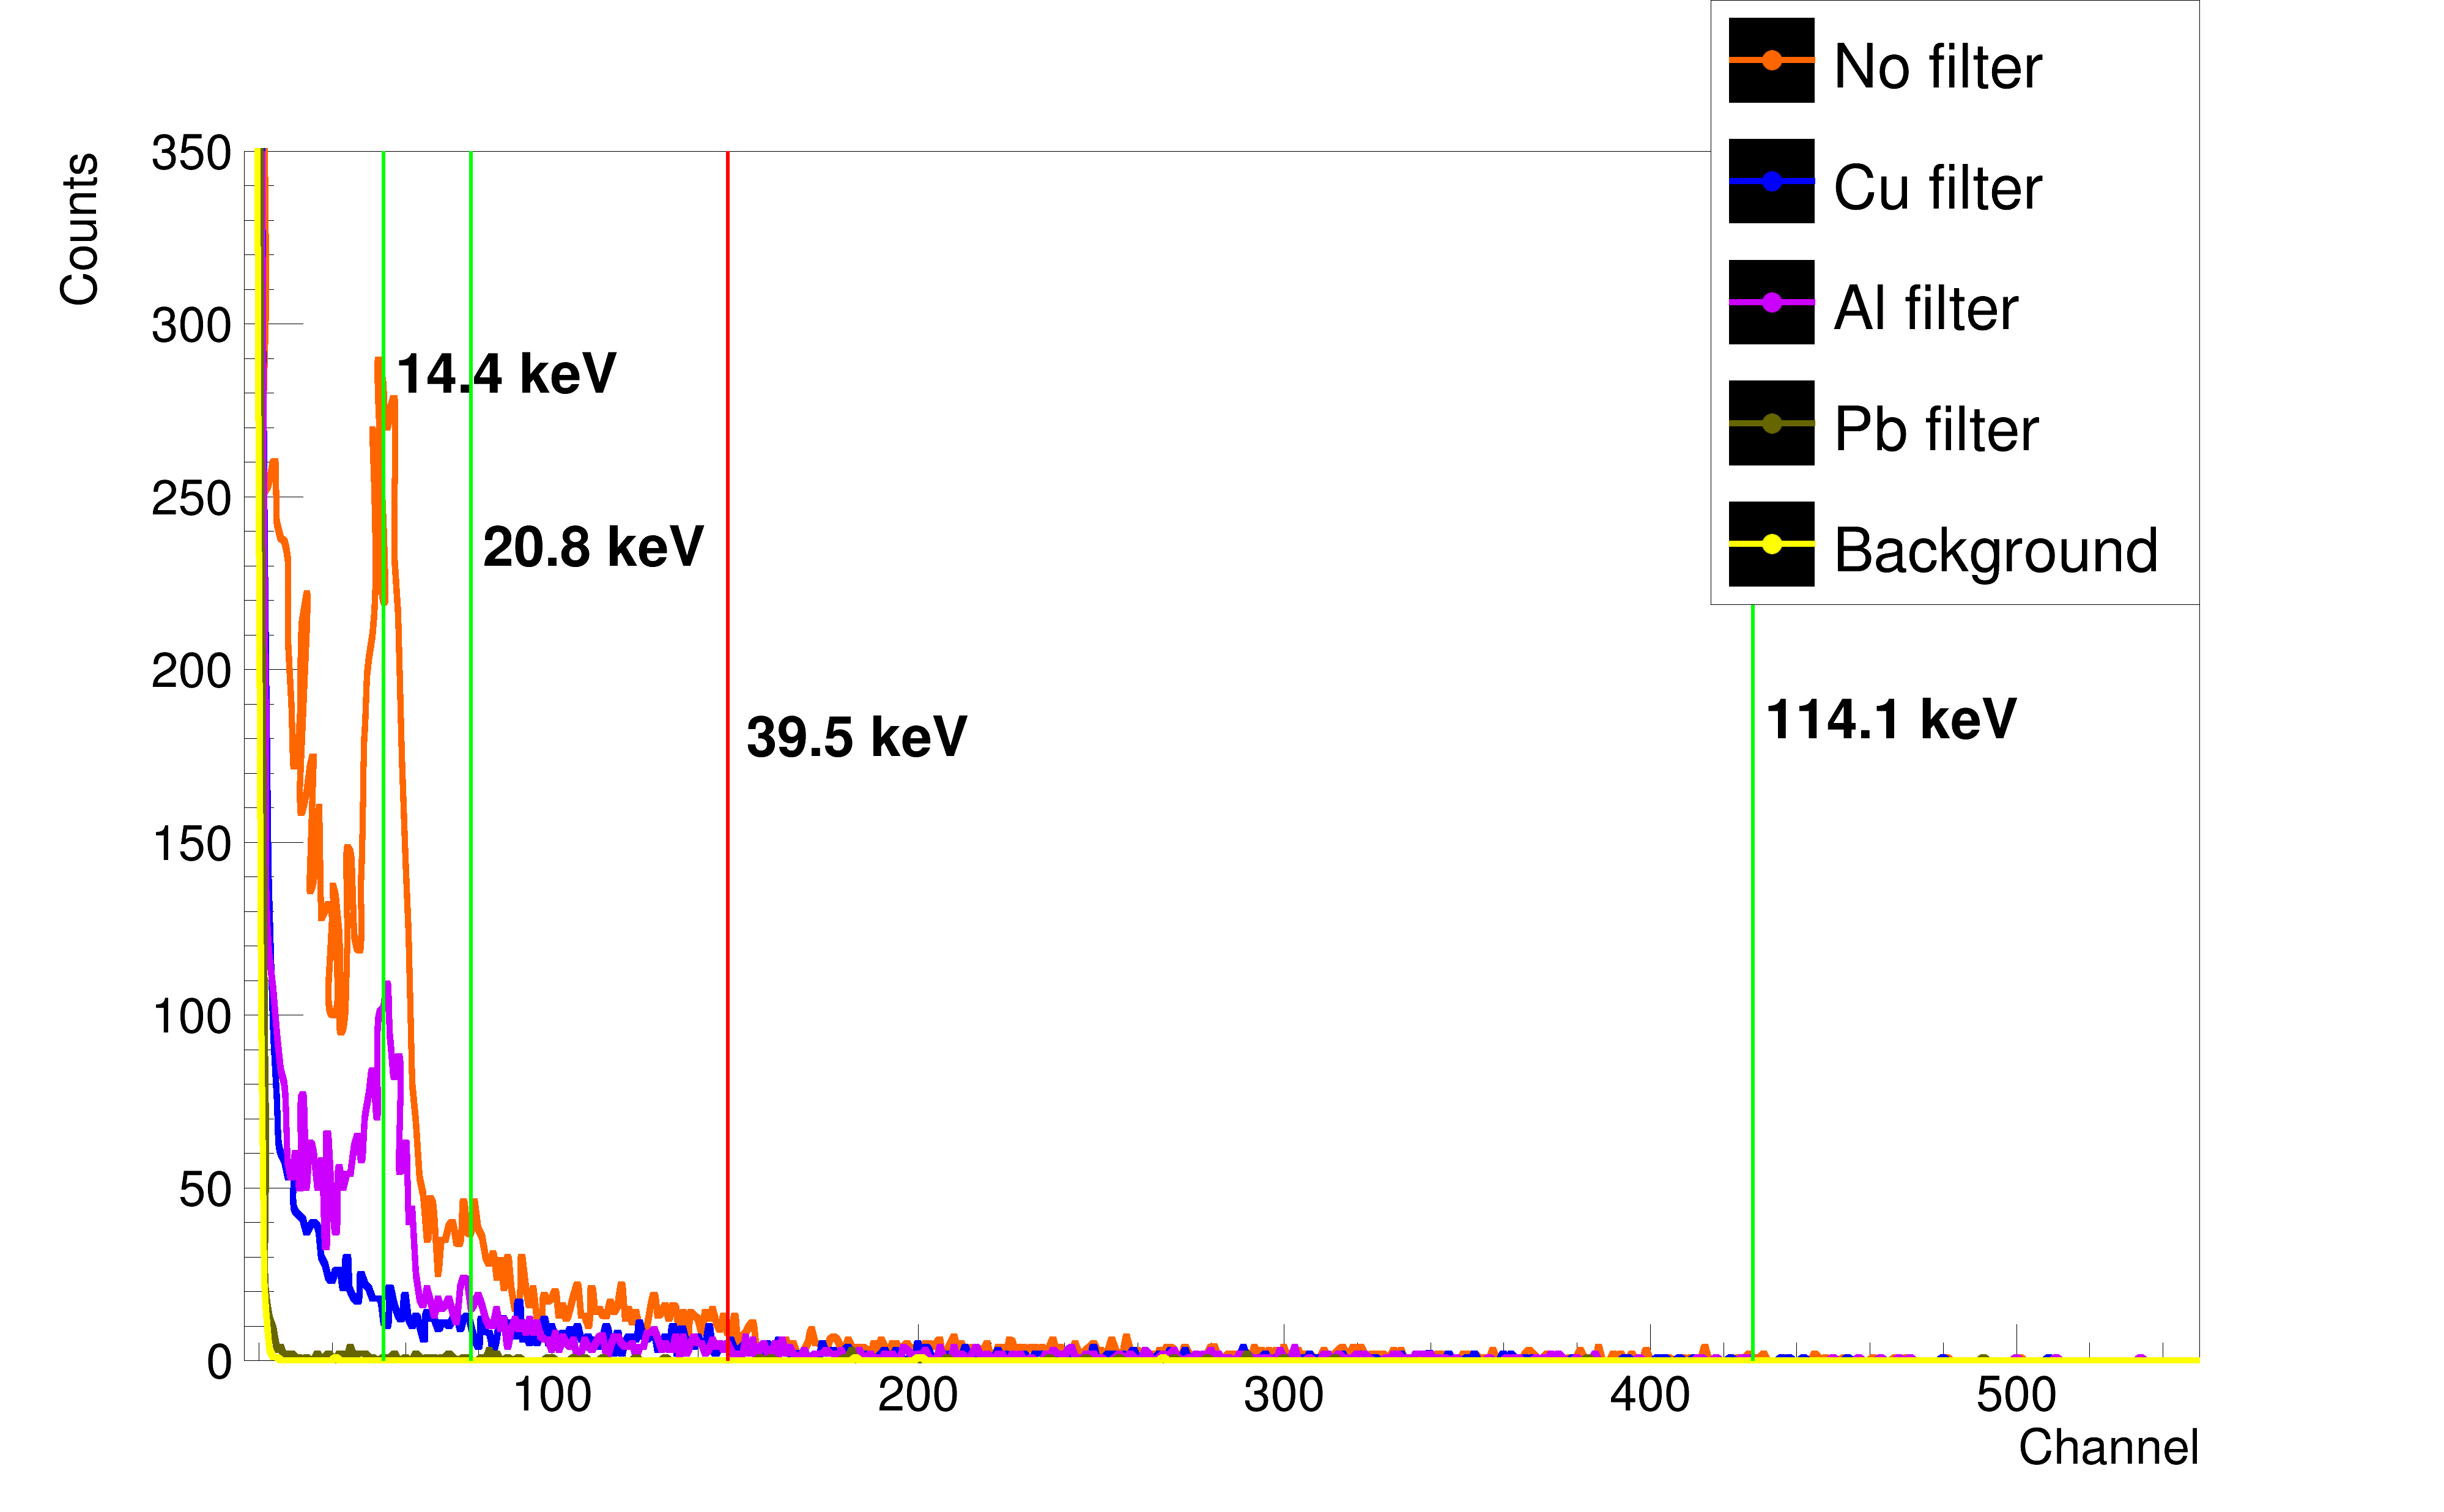
\includegraphics[scale=0.125, angle = 0]{./pictures/OPF430GammaTest.png}
 \caption{OPF430 spectra with founded energy peaks (green lines) and predicted Compton edge (red line).}
 \label{OPF430 spectra}
 
\end{figure}
It can be seen that the count rates are still much lower compared to previous photodiodes. This is probably due to the fact that the detector area is very small. The conclusion is that the OPF430 is capable of capturing the low energy gamma rays, but the efficiency is so bad that it is unusable for any real gamma spectroscopy application.
%It can be seen that the count rates are still much lower in comparison with previous photodiodes. This is probably due to the fact, that the surface of detector is very small. The conclusion is that OPF430 is capable of capturing the low-energy gamma rays, however, the efficiency is so bad that it makes it unusable for any real gamma spectroscopy application.
